\documentclass[9pt,twocolumn,twoside,lineno]{pnas-new}
% Use the lineno option to display guide line numbers if required.
% Note that the use of elements such as single-column equations
% may affect the guide line number alignment.

\newboolean{preprint}
\setboolean{preprint}{true}

\setboolean{displaywatermark}{false}

% Remove PNAS page styling (except first page, see below)
% for preprint
\ifthenelse{\boolean{preprint}}%
{%
\pagestyle{plain} % Reset page style
\renewcommand{\significancestatement}[1]{\relax} % Remove 'significance statement' box
}{}


% Used to adjust subfloat vertical alignment
\usepackage[export]{adjustbox}

% Easier float positions
\renewcommand{\topfraction}{0.9}	% max fraction of floats at top
\renewcommand{\bottomfraction}{0.8}	% max fraction of floats at bottom
%   Parameters for TEXT pages (not float pages):
\setcounter{topnumber}{2}
\setcounter{bottomnumber}{2}
\setcounter{totalnumber}{4}     % 2 may work better
\setcounter{dbltopnumber}{2}    % for 2-column pages
\renewcommand{\dbltopfraction}{0.9}	% fit big float above 2-col. text
\renewcommand{\textfraction}{0.07}	% allow minimal text w. figs
%   Parameters for FLOAT pages (not text pages):
\renewcommand{\floatpagefraction}{0.7}	% require fuller float pages
% N.B.: floatpagefraction MUST be less than topfraction !!
\renewcommand{\dblfloatpagefraction}{0.7}	% require fuller float pages

%Macros
\usepackage{xspace}
\usepackage{booktabs}
\usepackage{multirow}
\usepackage{amsmath,amsthm,mathtools}

% \usepackage{algorithm}
% \usepackage{algorithmic}
\renewcommand{\algorithmicrequire}{\textbf{Input:}}
\renewcommand{\algorithmicensure}{\textbf{Output:}}

\newcommand{\algoref}[1]{\hyperref[#1]{Algorithm~\ref*{#1}}}
\newcommand{\appendixref}[1]{\hyperref[#1]{Appendix~\ref*{#1}}}
\newcommand{\ie}{{i.e.}\xspace}
\newcommand{\eg}{{e.g.,}\xspace}
\newcommand{\cf}{{c.f.}\xspace}
\newcommand{\ea}{{et~al.}\xspace}
\newcommand{\aka}{{a.k.a.}\xspace}
\newcommand{\etc}{{etc.}\xspace}

\newcommand{\red}[1]{\textit{\color{red}{#1}}}
\usepackage{subfig}

\newtheorem{lemma}{Lemma}
\newtheorem{prop}{Proposition}
\newtheorem{theorem}{Theorem}
\newtheorem{corollary}{Corollary}
\newtheorem{observation}{Observation}
\newtheorem{proposition}{Proposition}
%\newtheorem*{claim}{Claim}
\newtheoremstyle{case}
  {\topsep}   % ABOVESPACE
  {\topsep}   % BELOWSPACE
  {}  % BODYFONT
  {\parindent}       % INDENT (empty value is the same as 0pt)
  {\bfseries} % HEADFONT
  {\normalfont.}         % HEADPUNCT
  {5pt plus 1pt minus 1pt} % HEADSPACE
  {#1 #2: {\normalfont #3}}          % CUSTOM-HEAD-SPEC
\theoremstyle{case}
\newtheorem{case}{Case}
\newtheorem{subcase}{Case}
\numberwithin{subcase}{case}
\makeatletter%Make sure case-counter is reset in every environment
\@addtoreset{case}{lemma}
\@addtoreset{case}{theorem}
\@addtoreset{case}{corollary}
% \@addtoreset{case}{claim} % Does not work with thmtools!
\makeatother

\newcommand{\dist}{\ensuremath{\text{dist}}}
\def\maxindeg{\Delta^{\!-}}
\def\dir#1{\vec{#1}}

\newcommand*{\MARK}[1]{(#1)}

%Import macros


\def\Dvorak{Dvo\v{r}\'{a}k\xspace}
\def\F{\ensuremath{\mathcal{F}}}


\newcommand{\piece}{piece\xspace} %other suggestions: parts, sections
\newcommand{\pieces}{pieces\xspace} %other suggestions: parts, sections
\newcommand{\podarref}{\texttt{podar-ref}\xspace}
\newcommand{\podarv}{\texttt{podarV}\xspace}
\newcommand{\hu}{\texttt{HuSB1}\xspace}
\newcommand{\sgc}{\textsf{spacegraphcats}\xspace}
\newcommand{\plass}{Plass\xspace}


\templatetype{pnasresearcharticle} % Choose template
% {pnasresearcharticle} = Template for a two-column research article
% {pnasmathematics} = Template for a one-column mathematics article
% {pnasinvited} = Template for a PNAS invited submission

% Turn this on for easier proofreading
% \usepackage{setspace}
% \doublespacing

\title{Exploring neighborhoods in large metagenome assembly graphs reveals hidden sequence diversity}

% Use letters for affiliations, numbers to show equal authorship (if applicable) and to indicate the corresponding author
\author[a,1]{C. Titus Brown}
% ORCID: 0000-0001-6001-2677
\author[b]{Dominik Moritz}
% ORCID: 0000-0002-3110-1053
\author[c]{Michael P. O'Brien}
% ORCID: 0000-0002-5942-791X
\author[c]{Felix Reidl}
% ORCID: 0000-0002-2354-3003
\author[a]{Taylor Reiter}
% ORCID: 0000-0002-7388-421X
\author[c,1]{Blair D. Sullivan}
% ORCID: 0000-0001-7720-6208

\affil[a]{Department of Population Health and Reproduction, University of California Davis}
\affil[b]{Paul G. Allen School of Computer Science and Engineering, University of Washington}
\affil[c]{Department of Computer Science, NC State University}

% Please give the surname of the lead author for the running footer
\leadauthor{Brown}

% Please add here a significance statement to explain the relevance of your work
\significancestatement{Authors must submit a 120-word maximum statement about the significance of their research paper written at a level understandable to an undergraduate educated scientist outside their field of speciality. The primary goal of the Significance Statement is to explain the relevance of the work in broad context to a broad readership. The Significance Statement appears in the paper itself and is required for all research papers.}

% Please include corresponding author, author contribution and author declaration information
\authorcontributions{DM, MPO, FR, and BDS designed and implemented algorithms; CTB, DM, MPO, and FR developed software; CTB and TR conducted biological data analysis; CTB and BDS supervised work. All authors interpreted results, wrote text, created figures, and approved the submitted paper.}
%\authordeclaration{Please declare any conflict of interest here.}
\correspondingauthor{\textsuperscript{1}To whom correspondence should be addressed. E-mail: ctbrown@ucdavis.edu, vbsulliv@ncsu.edu}

% Keywords are not mandatory, but authors are strongly encouraged to provide them. If provided, please include two to five keywords, separated by the pipe symbol, e.g:
\keywords{metagenomics $|$ sequence assembly $|$ strain variation $|$ bounded expansion $|$ dominating set}
\begin{abstract}
  Genomes computationally inferred from large metagenomic data sets
  are often incomplete and may be missing functionally important
  content and strain variation.  We introduce an information retrieval
  system for large metagenomic data sets that exploits the sparsity of
  DNA assembly graphs to efficiently extract subgraphs surrounding an
  inferred genome. We apply this system to recover missing content from
  genome bins and show that substantial genomic sequence variation is
  present in a real metagenome. Our software implementation is available
  at \url{https://github.com/spacegraphcats/spacegraphcats} under the
  3-Clause BSD License.
\end{abstract}

\dates{This manuscript was compiled on \today}
%\doi{\url{www.pnas.org/cgi/doi/10.1073/pnas.XXXXXXXXXX}}

\begin{document}

% Optional adjustment to line up main text (after abstract) of first page with line numbers, when using both lineno and twocolumn options.
% You should only change this length when you've finalised the article contents.
\verticaladjustment{-2pt}

\maketitle
\ifthenelse{\boolean{preprint}}%
{\thispagestyle{plain}}% Preprint style
{\thispagestyle{firststyle}}% Default PNAS first-page style
\ifthenelse{\boolean{shortarticle}}{\ifthenelse{\boolean{singlecolumn}}{\abscontentformatted}{\abscontent}}{}

%% THIS IS THE INTRODUCTION

%% Problem description and related work in the area of organizing large graphs.
%% Intro & citations should indicate to an editor appropriate potential reviewers.
%% Try to balance the novelty of hierarchy of dominating sets and efficient computation with
%% idea of using graph locality to improve binning.
\dropcap{M}etagenomics is the analysis of microbial communities through shotgun
DNA sequencing, which randomly samples many subsequences (reads)
from the genomic DNA of each microbe present in the community \cite{Quince2017}.

A common problem in metagenomics is the reconstruction of
individual microbial genomes from the mixture.
Typically this is
done by first running an assembly algorithm that reconstructs
longer linear regions based on a graph of the sampled
subsequences~\cite{pell2012scaling}, and then binning assembled
contigs together using compositional features and gene content~\cite{laczny2017busybee,lin2016accurate}.  These
``metagenome-assembled genomes'' are then
analyzed for phylogenetic markers and metabolic function. In recent years,
nearly 200,000 metagenome-assembled genomes have been published,
dramatically expanding our view of microbial life
\cite{Parks2017,Tully2018,Stewart2018,Delmont2018,Hug2016,Pasolli2019}.

Information present in shotgun metagenomes is often omitted from the
binned genomes due to either a failure to
assemble \cite{CAMI,Awad155358} or a failure to bin.  The underlying
technical reasons for these failures include low coverage, high
sequencing error, high strain variation, and/or sequences with
insufficient compositional or genic signal.  Recent work has
particularly focused on the problem of strain confusion, in which high
strain variation results in considerable fragmentation of assembled
content in mock or synthetic communities \cite{CAMI,Awad155358}; the
extent and impact of strain confusion in real metagenomes is still
unknown but potentially significant - metagenome-assembled genomes may be missing 20-40\% of true content \cite{brownstrain,Brito2016,baltic}.\looseness-1

%TER "fragmentation of assembled content" -- strain variation breaks the assembly, which results in smaller contigs that cannot be binned.
Associating unbinned metagenomic sequence to inferred bins or known
genomes is technically challenging.  Some approaches use mapping or
k-mer baiting, in which assembled sequences are used to extract reads
or contigs from a metagenome or
graph \cite{desman,Nayfach2016,ekg,mspminer,Petersen2016}.
These
methods fail to recover genomic content that does not directly overlap
with the query, such as large indels or novel genomic
islands. Moreover, most assembly graphs undergo substantial heuristic
error pruning and may not contain relevant content
\cite{CAMI,Awad155358}.
Graph queries have shown promise for recovering sequence from regions that do
not assemble well but are graph-proximal to the query \cite{metacherchant,perchlorate}. However, many graph query
algorithms are NP-hard and hence computationally intractable in the
general case; compounding the computational challenge, metagenome assembly
graphs are frequently large, with millions of nodes, and require 10s
to 100s of gigabytes of RAM for storage.\looseness-1

In this paper, we develop and implement a scalable graph query
framework for extracting unbinned sequence from metagenome assembly
graphs with millions of nodes. Crucially, we exploit the structural
sparsity of compact De Bruijn assembly graphs in order to compute a
succinct index data structure in linear time. We use this framework to
perform neighborhood queries in large assembly graphs, which enables
us to extract the genome of a novel bacterial species, recover missing
sequence variation in amino acid sequences for genome bins, and
identify missing content for metagenome-assembled genomes.  Our query
methods are assembly-free and avoid techniques that may discard strain
information such as error correction.  These algorithms are available
in an open-source Python software package,
\textsf{spacegraphcats}~\cite{spacegraphcats}.

% Add read graph mapping.


%This should be non-controversial.
\section*{Results}
%     #
%    # #   #       ####   ####  #####  # ##### #    # #    #
%   #   #  #      #    # #    # #    # #   #   #    # ##  ##
%  #     # #      #      #    # #    # #   #   ###### # ## #
%  ####### #      #  ### #    # #####  #   #   #    # #    #
%  #     # #      #    # #    # #   #  #   #   #    # #    #
%  #     # ######  ####   ####  #    # #   #   #    # #    #
%
%

%TODO: add legend for domset, etc colors in figure.
%TODO: smaller (a), (b), (c), (d)
% FIGURE 1
\begin{figure*}
 \centering
 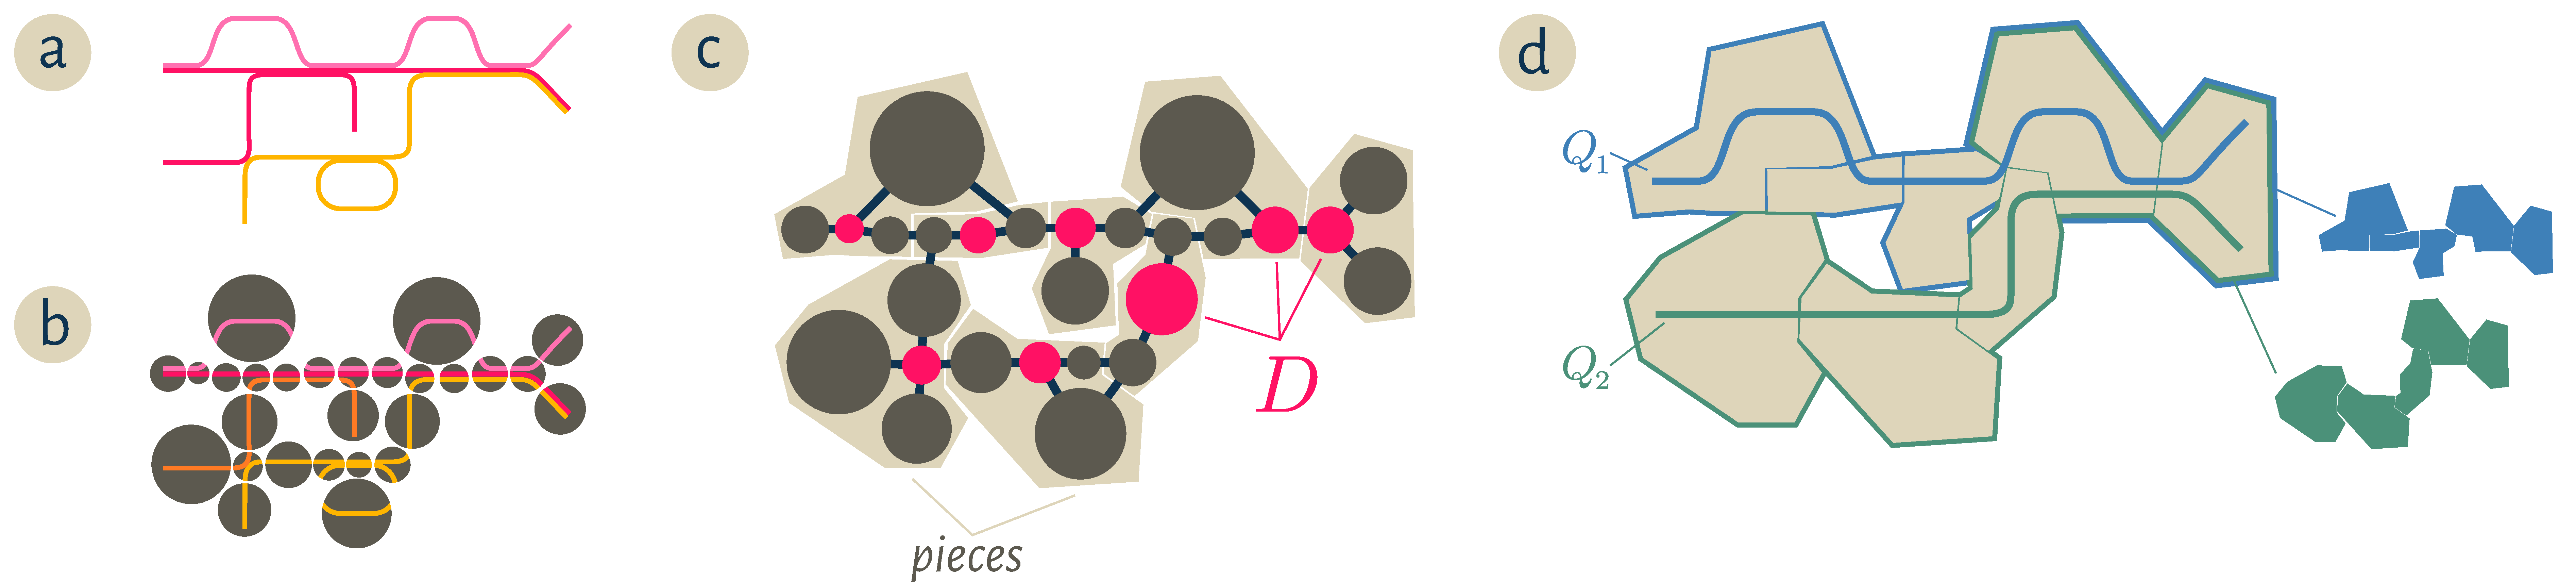
\includegraphics[width=\linewidth]{figures/domset}
	\caption{
 %(Reads ->) genomes -> DBG -> cDBG -> dominating set
 Starting from a collection of genomic sequences (\textbf a), we form an assembly graph
 where nodes represent distinct linear subsequences (\textbf b). In this assembly graph,
 known as a \emph{compact De Bruijn graph}~\cite{lin2016accurate}, nodes may
 represent many k-mers. The original genomic sequences correspond to walks in
 the graph, and shared nodes between the walks represent shared subsequences.
 %walk = path that can cross back on itself; maybe define in footnote?
 %didn't describe what happens at divergence points.
 We then (\textbf c) identify a subset of nodes $D$ called a \emph{dominating set} so that
 every node in the assembly graph is at distance at most one from some member of
 $D$ (marked pink). We further partition the graph into \emph{\pieces}
 by assigning every node to exactly one of the closest members of $D$ (beige regions
 in (\textbf c) and (\textbf d)).
 For a genomic query $Q$, the \emph{neighborhood} of $Q$ in this graph is the
 union of all \pieces which share at least one k-mer with the query. The colorful
 subsets of the pieces in (\textbf d) correspond to the neighborhoods of the
 queries $Q_1, Q_2$.
 }
 \label{fig:domset}
\end{figure*}

\subsection*{Dominating sets enable efficient neighborhood queries in large assembly graphs}

We designed and implemented~\cite{spacegraphcats} a set of algorithms for efficiently
finding content in a metagenome that is close to a query as measured
by distance in a compact De Bruijn graph (cDBG) representation of the
sequencing data (\autoref{fig:domset}). To accomplish this, we organize the cDBG into {\em \pieces}
around a set of \emph{dominators} that are collectively close to all vertices. In this
context, the {\em neighborhood} of a query is the union of all \pieces it overlaps;
to enable efficient search, we build an invertible index of the \pieces.

We compute dominators so that the minimum distance from every vertex
in the cDBG to some dominator is at most $r$ (an \emph{$r$-dominating set})
using~\algoref{alg:r-domset}, which is based on the linear-time approximation algorithm
given by \Dvorak and Reidl~\cite{felixThesis}. Although finding a minimum $r$-dominating set is
NP-hard~\cite{karp1972reducibility,chlebik2008approximation,downey2012parameterized} and
an approximation factor below~$\log n$ is probably impossible~\cite{chlebik2008approximation}
in general graphs, our approach guarantees constant-factor approximations
in linear running time by exploiting the fact that
(compact) De Bruijn graphs have \emph{bounded expansion}, a special type of
sparsity~\cite{sparsity}. \algoref{alg:r-domset} first
annotates the graph to determine the distances between all pairs of vertices at
distance at most $r$ (lines~\ref{algstep:dtf_start}-\ref{algstep:dtf_end}) and
then uses these distances to ensure each vertex is close to a dominator.
The core of the efficient distance computation is based on
\emph{distance-truncated transitive fraternal (dtf) augmentations}~\cite{felixThesis}
which produce a directed graph in which each arc $uv$ is labeled with
$\omega(uv)$, the distance from $u$ to $v$ in the original cDBG.\looseness-1

Importantly, our implementation enhances the algorithm
in~\cite{felixThesis} by computing only $r{-}1$ rounds of dtf-augmentations
instead of~$2r{-}1$. Since augmentation is the computationally most
expensive part of the pipeline and the running time depends non-linearly on
the number of rounds, this vastly improves this algorithm's scalability.
To maintain approximation guarantees on the dominating set size with fewer augmentations,
we introduce a threshold parameter $\texttt{domThreshold}(r)$
which affects the constant factor in our worst-case bound.
We selected a threshold (see Supp. Material) that produces $r$-dominating sets of
comparable size to those computed by the algorithm in~\cite{felixThesis}. Additionally,
we found that processing vertices using a minimum in-degree ordering (line~\ref{algstep:order})
was superior to other common orders (e.g. arbitrary, min/max total degree, max in-degree).\looseness-1

\begin{algorithm}[!b]
	\begin{algorithmic}[1]
		\Require Graph $G$, radius $r$
		\Ensure $r$-dominating set $D$ of $G$
		\State $\vec G_1\leftarrow \texttt{orient}(G)$\label{algstep:dtf_start}
		\For{$i\in 2,\dots, r$}
			\State $\vec G_i\leftarrow \texttt{dtfAugmentation}(\vec G_{i-1})$\label{algstep:dtf_end}
		\EndFor
		\State Initialize $d[v] \leftarrow \infty$ and $c[v] \leftarrow 0$ for all~$v \in G$
		\State $D\leftarrow \emptyset$
		\ForAll{$v\in \vec G_r$ sorted by ascending in-degree}\label{algstep:order}
			\ForAll{$u\in N^{-}(v)$} \label{algstep:pull-loop}
				\State $d[v]\leftarrow\operatorname{min}\left(d[v], d[u]+\omega(uv)\right)$\label{algstep:pull}
			\EndFor
			\If{$d[v]>r$}
				\State $D\leftarrow D\cup \{v\}$ and
					   $d[v]\leftarrow 0$\label{algstep:add_to_domset}\label{algstep:D1}
				\ForAll{$u\in N^-(v)$}\label{algstep:pushloop}
					\State $d[u]\leftarrow \operatorname{min}\left(d[u],\omega(uv)\right)$\label{algstep:push}
					\State $c[u]\leftarrow c[u] + 1$
					\If{$c[u] > \texttt{domThreshold}(r)$}
						\State $D\leftarrow D\cup \{u\}$ and
							   $d[u]\leftarrow 0$\label{algstep:D2}
						\ForAll{$w\in N^-(u)$}
							\State $d[w]\leftarrow \operatorname{min}\left(d[w],\omega(wu)\right)$\label{algstep:D2end}
						\EndFor
					\EndIf
				\EndFor
			\EndIf
		\EndFor
		\State \Return $D$
	\end{algorithmic}
	\caption{$\texttt{rdomset}(G, r)$}\label{alg:r-domset}
\end{algorithm}


After computing an $r$-dominating set $D$ of $G$ with \algoref{alg:r-domset},
\algoref{alg:index_pieces} partitions the vertices of $G$ into pieces so that
each \piece $P[v]$ contains a connected set of vertices for which $v$ is the
closest member of $D$ (\autoref{fig:domset}). Finally, we use minimal perfect
hashing (\texttt{mphfIndex})~\cite{limasset2017mphf} to compute an invertible
index\footnote{an invertible function that defines both an index and the corresponding inverted index}
between \pieces and their sequence content in the metagenome.

One feature of this approach is that the dominating set and index only need to be computed once for a given metagenome, independent of the number and content of anticipated queries.
Queries
can then be performed using \algoref{alg:search} in time that
scales linearly with the size of their {\em neighborhood} --
all genomic content assigned to \pieces that contain part of the query.

Our implementations of these algorithms in \sgc can be run on
metagenomic data with millions of cDBG nodes (\autoref{tab:data});
indexing takes under an hour, enabling queries to complete in seconds
to minutes (\autoref{tab:benchmarking}). See \appendixref{subsec:runtimes}
for full benchmarking (including cDBG construction). This
provides us with a tool to systematically investigate assembly graph
neighborhoods.

% can collapse lines 11-12 and 17-18 similar to line 5 for space saving if necessary
\begin{algorithm}[!h]
	\begin{algorithmic}[1]
		\Require{Metagenome $\mathcal{M}$, radius $r$}
		\Ensure{Invertible index $I \colon \mathcal{M} \to \mathcal{P}$; $\mathcal{P}$ is a set of \pieces}
		\State $G\leftarrow \texttt{cDBG}(\mathcal{M})$\;
		\State $D\leftarrow \texttt{rdomset}(G, r)$\;
		\State Initialize $\delta[v] \leftarrow v$ for all $v \in D$\;
		\State $U \leftarrow V(G) \setminus D$
		\While{$U \neq \emptyset$}\label{algstep:partition_start}
			\For{$v \in V(G) \setminus U$}
				\For{$u \in N(v) \cap U$}
					\State $\delta[u] \leftarrow \delta[v]$\;
					\State $U \leftarrow U \setminus \{u\}$\;
				\EndFor
			\EndFor
		\EndWhile
 		\State $\mathcal{P}[v] \leftarrow \{u:\delta[u] = v\}$\;\label{algstep:partition_end}
		\State $I_{\mathcal{M}} \leftarrow \texttt{mphfIndex}(\mathcal{M}, \mathcal{P})$\;
		\State \Return $I_{\mathcal{M}}$
	\end{algorithmic}
	\caption{$\texttt{indexPieces}(\mathcal{M},r)$}\label{alg:index_pieces}
\end{algorithm}

\begin{algorithm}[!h]
	\begin{algorithmic}[1]
		\Require Index $I_{\mathcal{M}}$, Query $Q$
		\Ensure The query neighborhood $\mathcal{N}_Q$
		\State $\mathcal{N}_Q \leftarrow \bigcup_{k \in Q}I_{\mathcal{M}}^{-1}(I_{\mathcal{M}}(k))$\;
		\State \Return $\mathcal{N}_Q$
	\end{algorithmic}
	\caption{$\texttt{search}(I_{\mathcal{M}}, Q)$}\label{alg:search}
\end{algorithm}


%Figure 2
\begin{figure*}
  \centering
  \subfloat{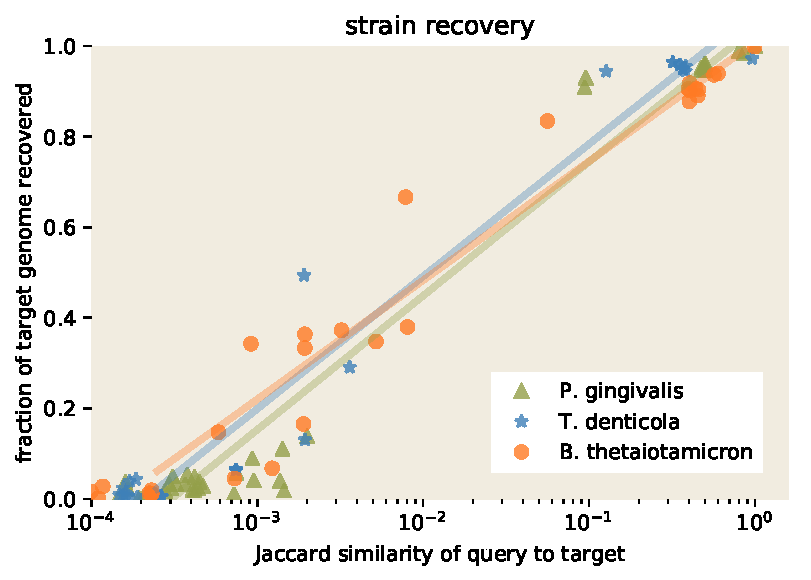
\includegraphics[width=0.4\linewidth,valign=c]{figures/partial_query_a}}%
  \hspace*{2cm}%
  \subfloat{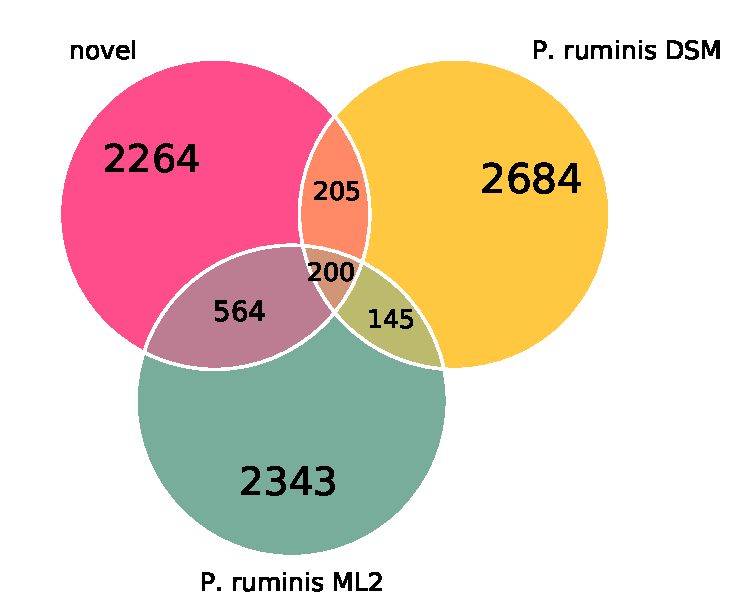
\includegraphics[width=0.3\linewidth,valign=c]{figures/partial_query_b}}%
  \hspace*{1cm}%
	\caption{Neighborhood queries enable recovery of relevant genomic content.
  (a) Left Panel: Recovery of each of three target genomes from \podarv
  using queries at a variety of Jaccard distances from the target. Recovery is
  calculated as containment of target genome in query neighborhood.
  (b) Right Panel: Recovery of novel {\em Proteiniclasticum } content
  from \podarv. Nucleotide content from two of the three known {\em P. ruminis} genomes
  overlapped approximately a megabase of sequence in the query neighborhood,
  which also contained approximately 2.3 Mbp of unknown sequence; the third known genome, {\em P. ruminis CGMCC}, was omitted from the figure as it is 99.7\% similar to {\em P. ruminis DSM}. Numbers are in thousands of k-mers.}\label{fig:partial_query}
\end{figure*}

%Data Set Properties

\begin{table}[t]
	\centering
	\begin{tabular}{l r r r r r}
	\toprule
	Dataset & $|V|$ & $|E|$/$|V|$ & $|D|$ & $\overline{|Q|}$ & $\overline{|\mathcal{P} \cap \mathcal{N}_Q|}$ \\
	\midrule
	\podarv &      916\,041 & 2.2 &    542\,350 & 1\,475\,892 &   4\,106 \\
	\hu     &  13\,852\,950 & 2.6 & 6\,724\,505 & 1\,112\,516 & 106\,091 \\
	\bottomrule
	\end{tabular}
	\caption{Number of cDBG nodes $|V|$, edge density of cDBG $|E|/|V|$, size of $1$-dominating set $|D|$,
	average query size (k-mers) $\overline{|Q|}$, and average number of pieces in query neighborhood $\overline{|\mathcal{P} \cap \mathcal{N}_Q|}$. Queries are the 51 genomes and 23 genome bins fully present in \podarv and \hu, respectively.} \label{tab:data}

	\centering
	\begin{tabular}{l l r r}
	\toprule
	Dataset & Algorithm & Time (s) & Memory (MB) \\
	\midrule
	\multirow{3}{*}{\podarv}
   & \texttt{rdomset}     &  78.1 &  4\,304 \\
   & \texttt{indexPieces} & 359.9 & 14\,108 \\
   & \texttt{search}      &  14.9 &  3\,463 \\
	\multirow{3}{*}{\hu}
   & \texttt{rdomset}     & 1\,181.1 & 60\,238  \\
   & \texttt{indexPieces} &    859.3 & 40\,713  \\
   & \texttt{search}      &     67.9 & 15\,228  \\
	\bottomrule
	\end{tabular}
	\caption{Time and memory usage of \sgc for Algorithms~\ref{alg:r-domset}-\ref{alg:search} on representative metagenome data. The times for \algoref{alg:search} are averaged over all queries (see \autoref{tab:data}).  Statistics reported for \algoref{alg:index_pieces} exclude lines 1-2 of pseudocode. Times are rounded to the nearest tenth of a second; memory is rounded to the nearest Megabyte.}\label{tab:benchmarking}
\end{table}


\subsection*{Neighborhood queries enable recovery of relevant unknown genomic content}
%Use queries that aren't 100% present in the graph to try to retrieve things that are there.

We first measured how well an inexact query can recover a target genome
from a metagenome. For a benchmark data set, we used the
\podarv data set \cite{podar}. This is a ``mock'' metagenome containing
genomes from 65 strains and species of bacteria and archaea, each
grown independently and rendered into DNA, then combined and sequenced
as a metagenome.  This metagenome is a commonly used
benchmark for assembly \cite{Awad155358,megahit,Seah2015,nurk2017metaspades}.

%by querying for a known target genome using queries closely related to the target.
To evaluate the effectiveness of neighborhood query at recovering
strain variants,
we chose three target genomes from \podarv -- {\em Porphyromonas
  gingivalis ATCC 33277}, {\em Treponema denticola ATCC 35405}, and
{\em Bacteroides thetaiotaomicron VPI-5482} -- that have many
taxonomically close relatives in GenBank. We then used these relatives
to query the \podarv mixture and measure the recovery of the target
genome.  The results, in \autoref{fig:partial_query}(a), show that
graph neighborhood query can recover 35\% or more of some target genomes
starting from a relative with Jaccard similarity as low as 1\%: even a
small number of shared k-mers sufficed to define a much larger neighborhood
that contains related genomes.


We next applied neighborhood query to retrieve an unknown genome from \podarv.
Several papers have noted the
presence of unexpected sequence in the assemblies of this data, and
Awad et al. identify at least two species that differ from
the intended mock metagenome contents \cite{megahit,Awad155358}.  One species
variant has partial matches to several different {\em
  Fusobacterium nucleatum} genomes, while the other incompletely matches to
three strains of
{\em Proteiniclasticum ruminis}.

The complete genomes of these two variants are not in public databases and, for
the {\em Proteiniclasticum} variant, cannot
be entirely recovered with existing approaches: when we
assemble the reads that share k-mers with the available genomes, a
marker-based analysis with CheckM estimates that 98.8\% of the {\em
  Fusobacterium} variant is recovered, while only 72.96\% of the {\em
  Proteiniclasticum} variant is recovered. We therefore tried using
neighborhood queries to expand our knowledge of the {\em Proteiniclasticum} variant.

We performed a neighborhood query into \podarv with all three known {\em
  Proteiniclasticum} genomes from GenBank.  We then extracted the reads
overlapping this neighborhood and assembled them with MEGAHIT.  The
retrieved genome neighborhood for {\em Proteiniclasticum} contains
2256K novel k-mers (\autoref{fig:partial_query}(b)). The reads from
the query neighborhood assembled into a 3.1 Mbp genome bin. The
assembly is estimated by CheckM to be 100\% complete, with 10.3\%
contamination.
The mean amino acid identity between {\em P. ruminis ML2} and the
neighborhood assembly is above 95\%, suggesting that this is indeed
the genome of the {\em Proteiniclasticum} variant, and that
neighborhood query retrieves a full draft genome sequence (see Supp. Material~\ref{subsec:aai}).

% FIGURE 3
\begin{figure*}[th]
	\centering
    \subfloat{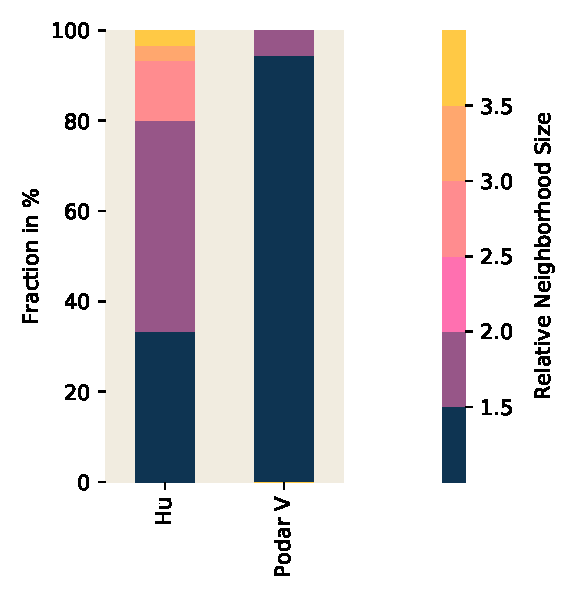
\includegraphics[width=0.34\linewidth]{figures/hu_strain_a}}
    \hspace{.05\linewidth}
    \subfloat{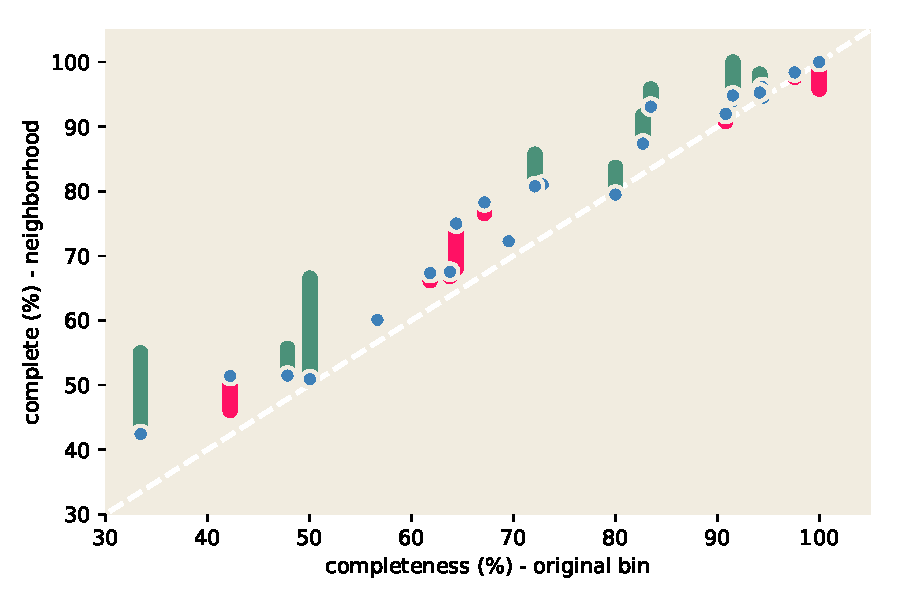
\includegraphics[width=0.55\linewidth]{figures/hu_strain_b}}
	\caption{Query neighborhoods in \hu metagenome are large and contain additional marker genes.
  (a) Left Panel: Neighborhood sizes are larger in \hu than in \podarv. Here
  we queried \podarv and \hu using each of 51 and 23 genomes fully present
  in the respective datasets and measured the relative size of its neighborhood—a
  size of 1 indicates that no additional sequence is present in the neighborhood,
  while a size of 2 indicates that the retrieved neighborhood is twice the size
  of the query genome.
  (b) Right Panel: Query neighborhoods are estimated to be more complete
  than the original genome bins. We queried \hu using each of 23 genomes binned
  from SB1, and assembled the resulting neighborhoods using MEGAHIT and \plass.
  The blue points represent completeness estimates of MEGAHIT-assembled
  neighborhoods, while green and pink bars represent the additional or missing
  content in the \plass assemblies respectively.
  }\label{fig:hu_strain}
\end{figure*}



\subsection*{Query neighborhoods in a real metagenome do not always assemble well}

Real metagenomes may differ substantially from mock metagenomes in
size, complexity, and content.  In particular, real metagenomes may
contain a complex mixture of species and strain variants \cite{Sharon2015}
and the performance of assembly and binning algorithms on these data sets
is challenging to evaluate in the absence of ground truth.
One recent comparison of single-cell genomes and metagenome-assembled
genomes in an ocean environment found that up to 40\% of single-cell
genome content may be missing in metagenome-assembled genomes \cite{baltic}.

We first ask whether genome query neighborhood sizes in a real
metagenome differ from mock metagenomes.  We examined genomes inferred
from the SB1 sample from the Hu et al.\ (2016) study, in which 6
metagenomic samples taken from various types of oil reservoirs were
sequenced, assembled, binned, and computationally analyzed for
biochemical function \cite{Hu2016}.  Examining the 23 binned genomes
in GenBank originating from the SB1 sample, we compared the \hu
neighborhood size distribution with the \podarv data set
(\autoref{fig:hu_strain}(a)). We saw that more genome bins in \hu
have 1.5x or larger query neighborhoods than do the genomes in
\podarv. This suggests the presence of considerably more local
neighborhood content in the real metagenome than in the mock
metagenome.

We next investigated metagenomic content in the query
neighborhoods.  As with the unknown variants in \podarv, we used
CheckM to estimate genome bin completeness.  The estimated bin
completeness for many of the query genomes is low
(\appendixref{subsec:checkm}).
To see if the query neighborhoods contain missing marker genes, we
assembled reads from the query neighborhoods using MEGAHIT.  However,
we found little improvement in the completion metrics (\autoref{fig:hu_strain}(b)).

Investigating further, we found that the query neighborhood assemblies
contain only between 4\% and 56\% of the neighborhood k-mer
content (\appendixref{subsec:inclusion}), suggesting that MEGAHIT is
not including many of the reads in the assembly of the query neighborhoods.
This could result from high
error rates and/or high strain variation in the underlying reads
\cite{CAMI,Awad155358}.

To attempt the recovery of more gene content from the assemblies, we turned to
the \plass amino acid assembler \cite{plass}. \plass implements an
overlap-based amino acid assembly approach that is considerably more
sensitive than nucleotide assemblers and could be more robust to
errors and strain variation \cite{spa}.

When we applied \plass to the reads from the query neighborhoods, we saw
a further increase in neighborhood completeness
(\autoref{fig:hu_strain}(b)).  This suggests that the genome bin
query neighborhoods contain real genes that are accessible to the
\plass amino acid assembler.  We note that these are unlikely to be
false positives, since CheckM uses a highly specific Hidden Markov Model
(HMM)-based
approach to detecting marker genes \cite{CheckM}.

%FIGURE 4
\begin{figure*}[!h]
	% \centering
    \subfloat{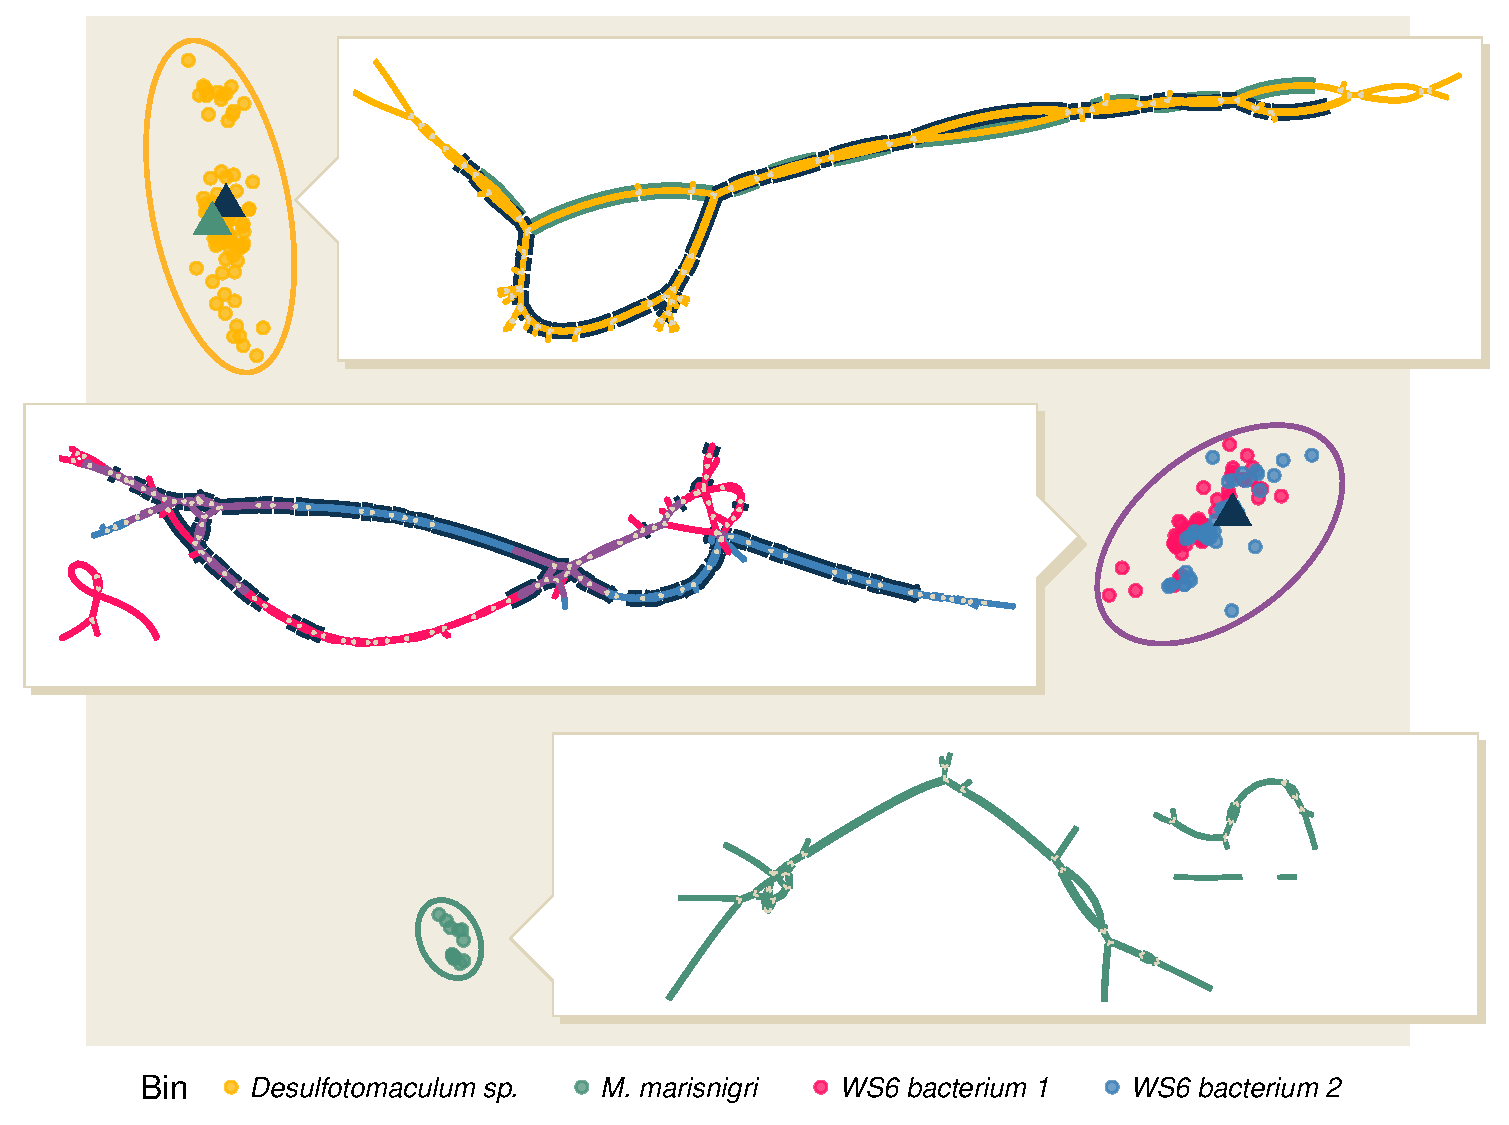
\includegraphics[width=0.54\linewidth]{figures/hu_content_a}}\hspace*{0.01\linewidth}%
    \subfloat{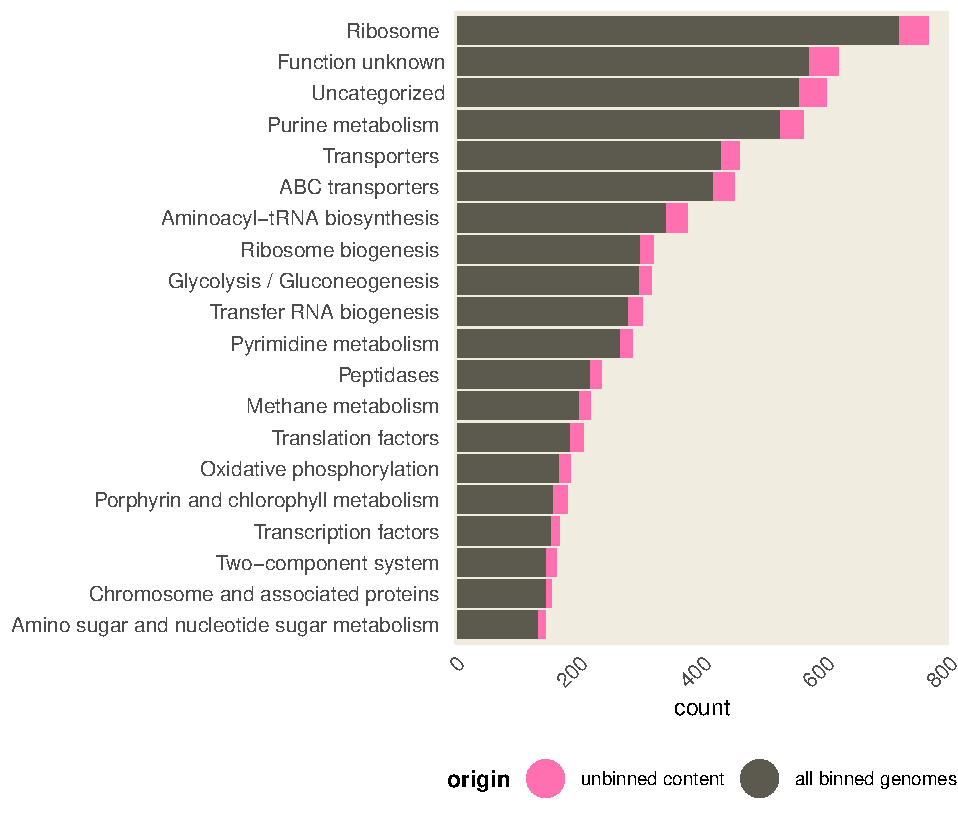
\includegraphics[width=0.45\linewidth]{figures/hu_content_b}}
    \caption{Query neighborhoods in \hu contain sequence variants and new genes.
      (a) Left Panel: gyrA has substantial minor sequence variation in several
      query neighborhoods. In this multidimensional scaling plot, each point
      represents a distinct gyrA sequence from the \plass assemblies of four
      representative query neighborhoods, colored by query binned genome.
      The triangles represent gyrA sequences originating from the
      query binned genome, if any are present.  The inlays
      are visualizations of assembly graphs of reads that contain {\em gyrA}
      sequence in each neighborhood. Unitigs are colored by their cluster of origin;
      matches to {\em gyrA} sequences from the bin are highlighted using color from relevant triangle.
      (b) Right Panel: Genome neighborhoods re-associate annotated
    functionality to binned genomes. For each of 23 genome bins
    originating from \hu, we found the unbinned content by removing all
    orthologs found in the binned genomes in \cite{hu} and by counting distinct
    ortholog annotations once. Functional content is
    distributed throughout pathways present in the binned genomes,
    and increases functionality associated with binned genomes by
    approximately 13\%.}
  \label{fig:hu_content}
\end{figure*}


\subsection*{Some query neighborhoods contain substantial strain variation}

If strain variation is contributing to poor nucleotide assembly of
marker genes in the query neigborhoods, then \plass should
assemble these variants into similar amino acid sequences.
Strain variation for unknown genes can be difficult to study due to
lack of ground truth, but highly conserved proteins should be readily
identifiable.

The {\em gyrA} gene encodes an essential DNA topoisomerase that
participates in DNA supercoiling and was used by \cite{Hu2016} as a
phylogenetic marker.  In the GenBank bins, we found that 15 of the 23
bins contain at least one gyrA sequence (with 18 {\em gyrA} genes
total).  We therefore used {\em gyrA} for an initial analysis of the
\plass-assembled neighborhood content for all 23 bins.  To avoid confounding effects of
random sequencing error in the analysis and increase specificity at the
cost of sensitivity, we focused only on high-abundance data:
we truncated all reads
in the query neighborhoods at any k-mer that appears fewer than five
times, and ran \plass on these abundance-trimmed reads from each
neighborhood.  We then searched the gene assemblies with a gyrA-derived
HMM, aligned all high-scoring matches, and calculated a pairwise similarity
matrix from the resulting alignment.\looseness-1
%TER add in k-mer size of 31 into materials and methods

When we examine all of the high-scoring gyrA protein matches in the
hard-trimmed data, we see
considerable sequence variation in some query neighborhoods
(\autoref{fig:hu_content}(a)). Much of this variation is present in
fragmented \plass assemblies; when the underlying nucleotide sequences
are retrieved and used to construct a compact De Bruijn graph, the
variation is visible as spurs off of a few longer paths (insets in
\autoref{fig:hu_content}(a)). When we count the number of
well-supported amino acid variants in isolated positions (i.e. ignoring linkage between variants)
we see that ten of the 23 neighborhoods have an increased number of gyrA
genes, with four neighborhoods gaining a gyrA where none exists in
the bin (\appendixref{subsec:gyrAnbhd}; see lowest inset
in \autoref{fig:hu_content}(a) for one example). Only one
neighborhood, {\em M. bacterium}, loses its gyrA genes due to the
stringent k-mer abundance trimming.
Collectively, the use of the \plass assembler on genome
neighborhoods substantially increases the number of gyrA sequences associated with bins.
% To calculate max # distinct gyrA, see code in misc/distinct_positions.ipynb.

We see this same pattern for many genes, including {\em alaS}, {\em gyrB},
{\em rpb2}
domain 6, {\em recA}, {\em rplB}, and {\em rpsC} (\appendixref{subsec:othergenes}).
This shows that multiple variants of those proteins are present within
at least some of the neighborhoods and implies the presence of
underlying nucleotide strain variation.
This strain variation may be
one reason that nucleotide assembly performs poorly: on average, only
19.6\% of \plass-assembled proteins are found within the nucleotide
assemblies.
% to calculate this number, see misc/plass-in-nucleotide-assemblies.md.

\subsection*{Query neighborhoods assembled with \plass contain additional functional content}

In addition to capturing variants close to sequences in the bins, we
identify many novel genes in the query neighborhoods. We used KEGG to
annotate the \plass-assembled amino acid sequences, and subtracted any
homolog already annotated in the genome bin.
We also ignoreed homolog abundance such that each homolog is counted only
once per neighborhood.

Novel functional content is distributed throughout pathways present in
the genome bins, and increases functionality associated with binned
genomes by approximately 13\% (\autoref{fig:hu_content}(b)).  This
includes orthologs in biologically relevant pathways
such as methane metabolism, which are important for biogeochemical
cycling in oil reservoirs \cite{Hu2016}.

Genes in these neighborhoods contain important metabolic functionality expanding
the pathways already identified in \cite{Hu2016}. We find 40
unique orthologs involved in nitrogen fixation across eight
neighborhoods, four of which had no ortholog in the bin.  Importantly,
we find the ratio of observed orthologs approximately matches that
noted in \cite{Hu2016}, where two thirds of nitrogen fixation
functionality is attributable to archaea (29 of 40 orthologs). This is
in contrast to most ecological systems where bacteria are the dominant
nitrogen fixers \cite{Hu2016}.


%This is where we can make subjective claims.
\section*{Discussion}
\subsection*{Efficient graph algorithms provide novel tools for investigating graph neighborhoods}

%This probably belongs in the introduction.
Recent work has shown that incorporating the structure of the assembly graph into the analysis of metagenome
data can provide a more complete picture of gene content \cite{perchlorate,metacherchant}. While this has provided evidence that it is
useful to analyze sequence that has small graph distance from a query (is in a ``neighborhood''), this approach
has not been widely adopted.
Na\"ively, local expansion around many queries in the assembly graph does not scale to these types of analyses
due to the overhead associated with searching
in a massive graph. The neighborhood index structure described in this work overcomes this computational
obstacle and enables rapid exploration of sequence data that is local to a query.

%In the past, biologists manually crafted genomic neighborhoods.
%SGC simplifies this dramatically by giving them a tool to query for neighborhoods of genomic sequences.
Because a partition into \pieces provides an implicit data reduction (the cDBG edge relationships are subsumed by \piece membership), the query-independent nature of the index allows many queries to be processed quickly without loading the entire graph into memory.
Our approach consequently provides a data exploration framework not otherwise available.

Exploiting the structural sparsity of cDBGs is a crucial component of our
algorithms. First, it is necessary to use graph structure to obtain a guarantee
that \algoref{alg:index_pieces} finds a small number of \pieces since the size
of a minimum $r$-dominating set cannot be approximated better than a factor of
$\log n$ in general graphs\footnote{That is, graphs about which we make no
structural assumptions.} unless $\text{NP}\subseteq \text{DTIME}(n^{O(\log \log
n)})$~\cite{chlebik2008approximation}. Without such a guarantee, we cannot be
sure that we are achieving significant data reduction by grouping cDBG vertices
into \pieces. Being able to do this in linear time also ensures that
indexing and querying can scale to very large data sets. Furthermore, because we
utilize a broad structural characterization (bounded expansion) of cDBGs rather than a
highly specialized aspect, our methods enable neighborhood-based
information retrieval in any domain whose graphs exhibit bounded expansion
structure; examples include some infrastructure,
social, and communication networks~\cite{demaine2014structural,felixThesis,wcol2018}.


% Novelty:
% * We create an index structure. k-mer -> piece -> bag of k-mers which is query-independent.
% * Inherent data reduction (neighborhoods are much smaller than the entire graph); we don't
% require you to load the entire graph in memory to do a single BFS. We only require you to load the
% neighborhoods.
%
% Theoretical Underpinning:
% * structural sparsity/efficient on sparse graphs
% * We run all experiments here with r = 1 (the simplest case; this already enables enough data reduction).
%
% Implementation:
% * There were several challenges in creating scalable effective algorithms and software.
% * summarize runtimes reported in results/supplement.
%
% Usability:
% * runtimes are reasonable relative to other analyses; scalability and memory usage.
% * Easy for biologists to use; integration with other pipelines? Designed as both Python API + standalone command-line tool.
% * You can explore your data by running lots of queries quickly. This isn't plausible in other paradigms.

\subsection*{Neighborhood queries extend genome bins}

In both the \podarv and \hu metagenomes, neighborhood queries were
able to identify additional content likely belonging to query genomes.
In the \podarv mock metagenome, we retrieved a potentially complete
genome for an unknown strain based on partial matches to known
genomes. In the \hu metagenome, we increased the estimated
completeness of most genome bins -- in some cases substantially,
e.g. in the case of {\em P\textunderscore bacterium 34\textunderscore 609}
we added an estimated 20.9\% to the genome bin.  In both cases we rely
solely on the structure of the assembly graph to expand the genome
bins. We do not make use of sequence composition, contig abundance, or
phylogenetic marker genes in our search. Thus graph proximity provides
an orthogonal set of information for genome-resolved metagenomics that
could be used to improve current binning techniques.

\subsection*{Query neighborhoods from real metagenomes contain substantial strain variation that may block assembly}

Previous work suggests that metagenome assembly and binning
approaches are fragile to strain variation \cite{CAMI,Awad155358}. This may
prevent the characterization of some genomes from metagenomes.  The extent of this problem is unknown, although
the majority of approaches to genome-resolved metagenomics rely on
assembly and thus could be affected.

In this work, we find that some of the sequence missing from genome
bins can be retrieved using neighborhood queries.  For \hu, some
genome bins are missing as many as 68.5\% of marker genes from the
original bins, with more than half of the 22 bins missing 20\% or
more; this accords well with evidence from a recent comparison of
single-cell genomes and metagenome-assembled genomes \cite{baltic}, in
which it was found that metagenome-assembled genomes were often
missing 20\% to 40\% of single-cell genomic sequence.  Neighborhood
query followed by amino acid assembly recovers additional content for
all but two of the genome bins; this is likely an underestimate, since
\plass may also be failing to assemble some content.

When we bioinformatically analyze the
function of the expanded genome content from neighborhood queries, our
results are consistent with the previous metabolic analyses by \cite{Hu2016}, and extend the
set of available genes by 13\%.
This suggests that current approaches to genome binning are specific,
and that the main question is sensitivity, which agrees with a more direct
measurement of lost content \cite{baltic}.

\subsection*{Neighborhood queries enable a genome-targeted workflow to recover strain variation}

The \sgc analysis workflow described above starts with genome bins. The
genome bins are used as a query into the metagenome assembly graph,
following which we extract reads from the query neighborhood.  We
assemble these reads with the \plass amino acid assembler, and then
analyze the assembly for gene content. We show that the \plass
assembly contains strain-level heterogeneity at the amino acid level,
and that this heterogeneity is supported by underlying nucleotide
diversity.  Even with stringent error trimming on the underlying
reads, we identify at least thirteen novel gyrA sequences in ten
genome neighborhoods.

Of note, this workflow explicitly associates the \plass assembled
proteins with specific genome bins, as opposed to a whole-metagenome
\plass assembly which recovers protein sequence from the entire
metagenome but does not link those proteins to specific genomes. The
binning-based workflow connects the increased sensitivity of \plass
assembly to the full suite of tools available for genome-resolved
metagenome analysis, including phylogenomic and metabolic
analysis. However, \sgc does not separate regions of the graph shared
in multiple query neighborhoods; existing
strain recovery approaches such as DESMAN or MSPminer could be used for this purpose
\cite{desman,mspminer}.

One future step could be to characterize unbinned genomic
content from metagenomes by looking at \plass-assembled marker genes
in the metagenome that do not belong to any bin's query neighborhood.
This would provide an estimate of the extent of
metagenome content remaining unbinned.


%Perhaps less-modest; definitely forward looking
\section*{Conclusions}
The neighborhood query approach described in this work provides an
alternative window into metagenome content associated with binned genomes. We extend previous work
showing that assembly-based methods are fragile to strain
variation, and provide an alternative workflow that substantially
broadens our ability to characterize metagenome content.  This first
investigation focuses on only two data sets, one mock and one real, but
the neighborhood indexing approach should be broadly applicable to
all shotgun metagenomes.

In this initial investigation of neighborhood indexing, we have
focused on using neighborhood queries with a genome bin.  We recognize
that this approach is of limited use in regions where no genome bin is
available; \sgc is flexible and performant enough to support
alternative approaches such as querying with k-mers belonging to genes
of interest.

Potential applications of \sgc in metagenomics include developing
metrics for genome binning quality, analyzing pangenome neighborhood
structure, exploring $r$-dominating sets for $r > 1$, extending analyses
to colored De Bruijn graphs, and investigating {\em de novo}
extraction of genomes based on neighborhood content.  We could also
apply \sgc to analyze the neighborhood structure of assembly graphs
overlayed with physical contact information (from e.g. HiC), which could
yield new applications in both metagenomics and genomics
\cite{Marbouty2014,Beitel2014}.

More generally, the graph indexing approach developed here may be
applicable well beyond metagenomes and sequence analysis.  The
exploitation of bounded expansion to efficiently compute $r$-dominating
sets on large graphs makes this technique applicable to a broad array
of problems.

(@checkme this content vs introduction; epxand introduction)



%WARNING: Using \verb inside matmethods macro causes strange errors about
%redefined $ and tikz-incompatibility! Widetext also seems to cause an error with
%ending scope of this stupid thing.
\matmethods{
\subsection*{Data}

We use two data sets: SRR606249 from
\texttt{podarV}~\cite{shakya2013comparative} and SRR1976948 (sample
SB1) from \texttt{hu}~\cite{hu}. Each data set was first preprocessed
to remove low-abundance k-mers as in \cite{Zhang2015}, using {\tt
  trim-low-abund.py} from khmer v2.1.2 \cite{Standage2017} with the
parameters {\tt -C 3 -Z 18 -M 20e9 -V -k 31}. We build compact De Bruijn
graphs using BCALM v2.2.0 \cite{bcalm}.  Stringent read trimming at
low-abundance k-mers was done with {\tt trim-low-abund.py} from khmer, with the
parameters {\tt -C 5 -M 20e9 -k 31}.

\subsection*{Software}

The source code for the index construction and search is available at
\url{https://github.com/spacegraphcats/spacegraphcats}~\cite{spacegraphcats}.
It is implemented in Python 3 under the 3-Clause BSD License.

Snakemake \cite{snakemake} workflows to reproduce all of the analysis
are available at
\url{https://github.com/dib-lab/2018-paper-spacegraphcats/}, and
Jupyter Notebooks to recreate all of the figures are in that same
repository \cite{jupyter}. The notebooks rely on the numpy,
matplotlib, pandas, scipy, and Vega-Lite libraries
\cite{numpy,matplotlib,pandas,scipy,vegalite}.

\subsection*{Benchmarking}

We measured time and memory usage for Algorithms 1-3 by executing the
following targets in the \sgc \texttt{conf/Snakefile}:
\texttt{catlas.csv} for \texttt{rdomset}, \texttt{contigs.fa.gz.mphf}
for \texttt{indexPieces}, and \texttt{search} for \texttt{search}.  We
report wall time and maximum resident set size, running under Ubuntu
18.04 on an NSF Jetstream virtual machine with 10 cores and 30 GB of
RAM \cite{jetstream1,jetstream2}. To measure maximum resident set
size, we used the memusg script (Jaeho Shin,
https://gist.github.com/netj/526585).

\subsection*{Graph denoising}

For each data set, we built a compact De Bruijn graph (cDBG) for
k=31 by computing the set of unitigs with
BCALM~\cite{chikhi2016compacting}, removing all vertices of degree one
with a mean $k$-mer abundance of 1.1 or less, and then contracting
long degree-two paths when possible.

\subsection*{Neighborhood indexing and search}

We use \sgc to build an $r$-dominating set for the denoised cDBG and
index it. We then perform neighborhood queries with \sgc, which
produces a set of cDBG nodes and reads that contributed to them.  The
full list of query genomes for the {\em Proteiniclasticum} query is
  available in Supp Material \ref{subsec:query_accessions}, and
  the NCBI accessions for the {\em P. gingivalis}, {\em T. denticola}, and {\em B. thetaiotamicron} queries are in the directory {\tt pipeline-base} of the paper repository, files {\tt strain-gingivalis.txt}, {\tt strain-denticola.txt}, and {\tt strain-bacteroides.txt}, respectively.

\subsection*{Search results analysis}

Query neighborhood size, Jaccard containment, and Jaccard similarity
was estimated using modulo hash signatures with a k-mer size of 31 and
a scaled factor of 1000, as implemented in sourmash v2.0a9
\cite{sourmash}.

\subsection*{Assembly and genome bin analysis}

We assembled reads using MEGAHIT v1.1.3 \cite{megahit} and \plass
v2-c7e35 \cite{plass}, treating the reads as single-ended. Bin
completeness was estimated with CheckM 1.0.11, with the {\tt
  --reduced\_tree} argument \cite{CheckM}.  Amino acid identity
between bins and genomes was calculated using CompareM commit
7cd51276 (https://github.com/dparks1134/CompareM).

\subsection*{Gene targeted analysis}

Analysis of specific genes was done with HMMER v3.2.1
\cite{hmmer}. \plass amino acid assemblies were queried with HMMER {\tt hmmscan}
 using the PFAM domains listed in Supp Material \ref{tab:pfam_accessions}, 
using a threshold score of 100 \cite{pfam}. Matching sequences were then
extracted from the assemblies for further analysis. To overcome
problems associated with comparing non-overlapping sequence fragments,
only sequences that overlapped 125 of the most-overlapped 200 residues
of the PFAM domain were retained (all sequences shared a minimum
overlap of 50 residues with all other sequences). These sequences were
aligned with MAFFT v7.407 with the {\tt --auto} argument \cite{mafft}. Pairwise similarities were
calculated using HMMER where the final value represented the number of
identical amino acids in the alignment divided by the number of
overlapping residues between the sequences. Pairwise distances were
visualized using a multidimensional scaling calculated in R using the
{\tt cmdscale} function. To visualize the assembly graph structure
underlying these amino acid assemblies, we use paladin v1.3.1 
to map abundance-trimmed reads back to the \plass amino acid assembly,
with the {\tt -f} argument set to 125 to set the minimum ORF length accepted \cite{paladin}. 
We extracted the reads that mapped to the gene of interest, created an
assembly graph using BCALM v2.2.0 \cite{chikhi2016compacting}, and
visualized the graph using Bandage v0.8.1 \cite{bandage}.

\subsection*{KEGG Analysis}

We annotated the \plass assemblies using Kyoto Encyclopedia of Genes
GhostKOALA v2.0 \cite{kegg}. To assign KEGG ortholog function, we used
methods implemented at https://github.com/edgraham/GhostKoalaParser
release 1.1.


}%end of matmethods

\showmatmethods % Display the Materials and Methods section


\acknow{This work is funded in part by the Gordon and Betty Moore
  Foundation’s Data-Driven Discovery Initiative through Grants
  GBMF4551 to C. Titus Brown, GBMF4553 to Jeffrey Heer, and GBMF4560
  to Blair D. Sullivan.  This work arose from the Barnraising for
  Data-Intensive Discovery at Mt. Desert Island Biological Lab in May
  2016.  We thank Erich Schwarz, Martin Steinegger, Johannes
  S{\"o}ding, Mark Blaxter, and members of the Data Intensive Biology
  lab at UC Davis for discussion and feedback.
 }%end of acknow

\showacknow % Display the acknowledgments section

% \pnasbreak splits and balances the columns before the references.
% If you see unexpected formatting errors, try commenting out this line
% as it can run into problems with floats and footnotes on the final page.
%\pnasbreak

% Bibliography
\bibliography{bibliography}

\newpage
\clearpage
\appendix

\section{Appendix}

\subsection{Notation}\label{app:notation} For a graph $G$
we write $V(G)$ and $E(G)$ for its vertex and edge set, respectively. For a
vertex $v \in V(G)$, we write $N(v)$ to denote its neighborhood, \ie the set
containing all vertices that are adjacent to it in $G$. We further
write $G-v$ for the graph obtained from $G$ by removing $v$ and all edges
incident to it.

For a directed graph (digraph) $\dir G$, we use $N^-(v)$ to denote
the \emph{in-neighborhood} of $v \in V(\dir G)$, that is, the set
of all vertices $w$ for which an arc $wv$ exists in $\dir G$. The
size of that in-neighbourhood is called the \emph{in-degree} of $v$.
We write $\maxindeg(\dir G)$ for the maximum in-degree over all
vertices of $\dir G$.
For ease of notation, we usually write ``$v \in G$'' instead of
``$v \in V(G)$'' and ``$uv \in G$'' instead of ``$\{u,v\} \in E(G)$''
(same for digraphs).

A vertex set~$S \subseteq V(G)$ is \emph{$r$-scattered} if all vertices
in it have pairwise distance at least~$r$ in~$G$. Note that if a set~$S$
is $(2r+1)$-scattered in~$G$, then no single vertex can $r$-dominate
more than one vertex of~$S$. It follows that any $r$-dominating set of~$G$ must
have size at least~$|S|$; we can therefore use $(2r+1)$-scattered sets to
prove lower bounds on the $r$-domination number of a graph.

\subsection{Dtf-augmentation}\label{app:dtf} For the sake
of completeness, we briefly describe how dtf-augmentations
$\dir G_1, \dir G_2, \ldots, \dir G_r$ are computed for an input
graph $G$.

First, the graph $\dir G_1$ is a \emph{minimum in-degree
orientation} of $G$ obtained as follows: we find a vertex~$u$ of
minimum degree in $G$, orient the incident edges towards $u$ and
the repeat the procedure in $G - u$ until no vertices remain.

Given $\dir G_i$, $i \geq 1$ we then compute $\dir G_{i+1}$ by
applying an \emph{augmentation step}:

\begin{enumerate}
    \item $\dir G_{i+1}$ contains all arcs of $\dir G_i$,
    \item if there is a pair of arcs~$uv \in \dir G_j$
          and $vw \in \dir G_k$ with $j + k = i + 1$, then
          we add $uw$ to $\dir G_{i+1}$,
    \item if there is a pair of arcs~$uv \in \dir G_j$
          and $wv \in \dir G_k$ with $j + k = i + 1$, then
          either the arc $uw$ or the arc $wu$ must be
          in $\dir G_{i+1}$.
\end{enumerate}
The ambiguity in the last step is resolved as follows:
we collect all edges $uw$ for which the last case applies
in a graph $H$ and then compute a minimum in-degree
orientation $\dir H$ of~$H$. We then add the arcs
in $\dir H$ to $\dir G_{i+1}$.

For ease of notation, we define $\omega(uv)$ to be the
smallest index $i \leq r$ such that $uv \in \dir G_i$
(and $\infty$ if no such index exists).
We make use of two crucial properties of dtf augmentations
in the following. First, vertices that have distance at most
$r$ in $G$ have distance at most two in $\dir G_r$:

\begin{lemma}[\cf Lemma 26 in~\cite{felixThesis}]
  For every pair $u,v \in G$ with $\dist(u,v) = d$ and
  for every integer~$r \geq d$ one of the following holds:
  \begin{enumerate}
    \item $uv \in \dir G_r$ and $\omega(uv) = d$,
    \item $vu \in \dir G_r$ and $\omega(vu) = d$,
    \item or there exists $x$ such that $xu, xv \in \dir G_r$ and
          $\omega(xu) + \omega(xv) = d$.
  \end{enumerate}
\end{lemma}

\noindent
Second, if we compute dtf-augmentations of graphs from a bounded
expansion class (to which graph of bounded maximum degree like
cDBGs belong), then the maximum in-degree
of its $r$th augmentation can be bounded by a function independent
of the \emph{size} of the graph:

\begin{theorem}[\cf Theorem 16 in~\cite{felixThesis}]\label{thm:dtf}
  For every graph class $\mathcal G$ with bounded expansion there exists
  a function~$f$ such that for every member $G \in \mathcal G$
  the $r$th dtf-augmentation $\dir G_r$ computed as above
  satisfies
  $\maxindeg(\dir G_r) \leq f(r)$.
\end{theorem}

\subsection{Approximation guarantee}\label{app:threshold}
% Note: labels don't work right now because we're not numbering subsections (style file issue)

Let us introduce some notation for the analysis of
Algorithm~\ref{alg:r-domset}. We first partition the vertices of~$D$ according
to whether they were added in line~\ref{algstep:D1} (denoted by~$D_1$) or in
line~\ref{algstep:D2} (denoted by~$D_2$). Let~$v_1,\ldots,v_n$ be the vertex-
order in which they are iterated over in the loop starting at
line~\ref{algstep:order}. We will use the notation~$D_1^i$, $D_2^i$, $d^i$,
and~$c^i$ to represent the states of the respective sets and data structures
during the $i$th iteration of said loop. Let~$\tau :=
\texttt{domThreshold}(r)$ be the chosen threshold (we discuss a good value
for $\tau$ on cDBGs below).

\begin{lemma}
  After the for-loop at line~\ref{algstep:pull-loop} has finished,
  \[
    d^i[v_i] = \begin{cases*}
      \dist_G(v,D^i) & if $\dist_G(v,D^i) \leq r$, and \\
      \infty & otherwise.
    \end{cases*}
  \]
\end{lemma}
\begin{proof}
  The statement trivially holds while~$D^i = \emptyset$, so assume otherwise.
  Let~$u_h \in D^i$ be the vertex closest to~$v_i$ and let~$h < i$
  be the iteration in which~$u_h$ was added to~$D$ (either in
  line~\ref{algstep:D1} or line~\ref{algstep:D2} of that iteration).

  If $d := \dist_G(v_i,u_h) > r$,
  then~$d^i[v_i]$ has not been changed yet and is still set to~$\infty$.
  Otherwise, consider the three possible scenarios promised by the
  distance-property of dtf-augmentations:

  \begin{case}[$v_iu_h \in \dir G_d$]
    Then~$\omega(v_iu_h) = d$ and in iteration~$h$
    the value of~$d^h[v_i]$ is set to the correct value~$d$
    at line~\ref{algstep:pull}.
    By assumption this distance remains minimal until iteration~$i$
    and hence~$d^i[v_i] = d^h[v_i] = d$.
  \end{case}

  \begin{case}[$u_hv_i \in \dir G_d$]
    Then~$\omega(v_iu_h) = d$ and in iteration~$i$
    the value of~$d^i[v_i]$ is set to the correct value~$d$
    at line~\ref{algstep:pull}.
  \end{case}

  % The cases env is a bit hacky. Parenthesis don't work well,
  % unless hidden in a macro.
  \def\ww#1{\omega(#1)}
  \begin{case}[$xu_h,xv_i \in \dir G_d$  with~$\ww{xu_h} + \ww{xv_i} = d$]\mbox{}\\
    During iteration~$h$ the value of~$d^h[x]$ is set to~$\ww{xu_h}$
    at line~\ref{algstep:pull} and subsequently retrieved
    in iteration~$i$ when $d^i[v_i]$ is set to
    \[
      d^i[x] + \ww{xu_h} = \ww{xu_h} + \ww{xv_i} = d.
    \]
    \vspace*{-1.5em}
  \end{case}
  \noindent
  We conclude that after the execution of the loop at line~\ref{algstep:pull}.
  $d^i[v_i]$ is set to~$\infty$ if~$v_i$ is not dominated by~$D_i$ and is
  otherwise set to~$\dist_G(v_i,D^i)$, as claimed.
\end{proof}

\noindent
As an immediate consequence, we see the conditional statement at the end of
the loop at line~\ref{algstep:pull} accurately determines whether $v_i$ is
dominated by~$D_i$ or not. Accordingly, line~\ref{algstep:D2}
of the loop is only executed if~$v_i$ is \emph{not} dominated by~$D^i$.
Another consequence is that all vertices in~$D_1$ have large distance to
each other:

\begin{corollary}
  The set~$D_1$ is $(r+1)$-scattered in~$G$.
\end{corollary}

\noindent
We need one more important property of the algorithm in order to derive
the approximation factor.

\begin{lemma}\label{lemma:D1-intersection}
  For every~$w \in G$ it holds that~$|D_1 \cap N^-_r(w)| \leq \tau+1$.
\end{lemma}
\begin{proof}
  Assume towards a contradiction that~$\tau+2$ such vertices
  $v_{i_1},\ldots,v_{i_\tau+2}$, $i_1 < i_2 < \ldots < i_{\tau+2}$ exist in~$D_1
  \cap N^-_r(w)$. Since every such vertex~$v_i$, $i \in \{i_1,\ldots
  i_{\tau+2}\}$, was added to~$D$ in part~\MARK{2}, part~\MARK{3} of the
  algorithm was executed during iteration~$i$ as well. Thus~$c[w]$ was
  increased in each iteration~$i$ and during iteration~$i_{\tau+1}$ we have that
  $c[w] \geq \tau + 1$ after the increment of~$c[w]$. Therefore part~\MARK{4}
  must have been executed for~$w$, including~$w$ into~$D$. Hence~$w \in D^s$
  for~$s > i_{\tau+1}$ and in particular $w \in D^{i_{\tau+2}}$. But then
  $v_{i_{\tau+2}}$ was dominated by~$w$ at the beginning of iteration~$i_{\tau+2}$
  since we assumed that~$\omega(rv_{i_{\tau+2}}) \leq r$, thus~$v_{i_{\tau+2}}$
  would not have been included in~$D$ at step~\MARK{2}. This contradicts our
  assumption of $v_{i_{\tau+2}} \in D_1$ so the claim must hold.
\end{proof}

\begin{lemma}
  There exists a subset~$A \subseteq D_1$ such that~$A$ is
  $(2r+1)$-scattered in~$G$ and
  \[
  	|A| \geq \frac{|D|}{2(\tau+2)\maxindeg(\dir G_{2r}))\maxindeg(\dir G_r)}.
  \]
\end{lemma}
\begin{proof}
  We construct an auxiliary graph~$H$ with vertices~$D_1$ by
  adding arcs~$v_iv_j$ for $v_i,v_j \in D_1$ with $i < j$
  whenever~$\dist_G(v_i,v_j) \leq 2r$.
  Let~$\dir G_{2r}$ be a $2r$th dtf-augmentation of~$G$ and
  let us create a digraph~$\dir H$ by orienting
  every edge~$uv \in H$ as follows:
  \begin{enumerate}
    \item If of~$uv,vu \in \dir G_{2r}$,
          then orient~$uv$ in~$\dir H$ according to the corresponding
          arc in $\dir G_{2r}$ (if both arcs exists choose an arbitrary
          orientation),
    \item otherwise there exists~$w \in N^-_{2r}(u) \cap N^-_{2r}(v)$
          with~$\omega_{2r}(u) + \omega_{2r}(v) = \dist_G(u,v) \leq 2r$. Orient the edge~$uv$ towards that vertex~$x \in \{u,v\}$
          for which~$\omega_{2r}(x)$ is larger.
  \end{enumerate}
  We now argue that~$\maxindeg(\dir H)$ is small. Consider any vertex $v \in
  \dir H$. Every in-arc $uv \in \dir H$ either is of type~1, of which we have
  at most~$\maxindeg(\dir G_{2r})$, or of type~2. Consider a group of in-
  arcs~$u_iv$, $1 \leq i \leq \ell$ of type~2 that are all present because of
  a common vertex~$w$. Since~$w \in N^-_{2r}(u)$, we have at
  most~$\maxindeg(\dir G_{2r})$ such groups. By construction,
  $\omega_{2r}(wu_i) \leq \omega_{2r}(wv)$ and since both weights sum to less
  than~$2r$, this means that~$\omega_{2r}(wu_i) \leq r$.
  Lemma~\ref{lemma:D1-intersection} now tells us that~$\ell \leq \tau + 1$.
  Therefore~$v$ has at most~$(\tau+1) \maxindeg(\dir G_{2r})$ in-arcs of type~2 and we conclude that
  \[
    \maxindeg(\dir H) \leq \maxindeg(\dir G_{2r}) + (\tau+1)\maxindeg(\dir G_{2r}) = (\tau+2)\maxindeg(\dir G_{2r}).
  \]
  This finally implies that~$H$ is $2(\tau+2)\maxindeg(\dir G_{2r})$-degenerate and therefore contains an independent set~$A \subseteq V(H)$
  of size at least~$|A| \geq |H| / (2(\tau+2)\maxindeg(\dir G_{2r}))$.
  Taken together with the fact that~$|H| = |D_1| \geq |D| / \maxindeg(\dir G_r)$
  (every vertex added to~$D_1$ will cause at most~$\maxindeg(\dir G_r)$ many
  vertices to be added to~$D_2$ in the loop at line~\ref{algstep:pushloop}
  and~$D = D_1 \cup D_2$), we find that
  \[
  	|A| \geq \frac{|D|}{2(\tau+2)\maxindeg(\dir G_{2r}))\maxindeg(\dir G_r)}
  \]
  By construction of~$H$ we conclude that~$A$ is $(2r+1)$-scattered
  in~$G$ of the claimed size.
\end{proof}

\noindent
Since a $(2r+1)$-scattered set provides a lower bound for an~$r$-dominating
set, we conclude that Algorithm~\ref{alg:r-domset} computes a
$2(\tau+2)\maxindeg(\dir G_{2r})\maxindeg(\dir G_r)$-approximation of an
optimal $r$-dominating set. In other words, we obtain a constant-factor
approximation in graphs of bounded expansion since the quantities $\maxindeg(\dir
G_{2r})\maxindeg(\dir G_r)$ are constants per Theorem~\ref{thm:dtf} in bounded
expansion classes and the quantity $2(\tau+2)$ is a constant of our choosing.

In practice one could, depending on the value of $\maxindeg(\dir G_r)$
and $\maxindeg(\dir G_{2r})$, compute the optimal value for~$\tau$ to minimize the
approximation guarantee. However, this
would necessitate the computation of $2r$ augmentation, the expensive step we
want to avoid. Alternatively, we can choose a `good enough' value for $\tau$
that still guarantees a constant-factor approximation while being easy to
determine in practice. In the context of cDBGs, we found that
$\tau := (2r)^2$ yields reliably good results.

\subsection{Computational Runtimes}
\label{subsec:runtimes}

See ``Benchmarking'' in Materials and Methods for benchmarking methods.

The \podarv data set was retrieved from the NCBI SRA using accession
SRR606249.  The full build and indexing of the 103 million
error-trimmed reads (10.3 Gbp in total) took approximately 23 minutes
and required 12.8 GB of RAM. Loading the indices for search required
4.3 GB of RAM and a search with a 3 Mbp genome took approximately 32
seconds.

The \hu data set was retrieved from the NCBI SRA using accession
SRR1976948. The full build and indexing of the 34 million
error-trimmed reads (8.5 Gbp in total) required approximately 217
minutes and required 24.4 GB of RAM. Loading the indices for search
required 18 GB of RAM and a search with a 3 Mbp genome took
approximately 80 seconds.

For data set complexity (number of k-mers, number of cDBG nodes) please see
Table~\ref{tab:data}.

\subsection{spacegraphcats pipeline overview}
\label{subsec:sgc_pipeline}

\textsf{spacegraphcats} follows a series of steps when run on sequencing
data, see Figure~\ref{fig:sgc_dag}. In detail, we perform the following
steps.

\emph{BCALM}. Use BCALM to generate a cDBG. Then convert a BCALM {\tt unitigs.fa}
output (a cDBG) into spacegraphcats files.
Outputs an undirected graph, a file containing the sequences, and a
{\tt .info.csv} file containing information about the contig. Also outputs
sourmash {\tt k=31}, {\tt scaled=1000} signatures for both input and
output files.

\emph{spacegraphcats.cdbg.label\_cdbg}. Build an index that can be
used to retrieve individual reads or contigs by cDBG node ID; produce
a SQLite database for fast retrieval. Briefly, this script creates a
sqlite database with a single table, {\tt sequences}, where a query like
{\tt SELECT DISTINCT sequences.offset FROM sequences WHERE label ...}
can be executed to return the offset of all sequences with the given
label; the offsets refer to BGZF coordinates in the gzipped sequence collection. Here, 'label' is the cDBG ID to which the sequence belongs.

The script {\tt extract\_reads\_by\_frontier\_sqlite.py} is a downstream script to
extract the reads with a frontier search.
Specifically: 1. walk through the contigs assembled from the cDBG;
2. build a DBG cover using khmer tags, such that every k-mer in the DBG is
within distance d=40 of a tag;  3. label each tag with the cDBG node ID
from the contig; 4. save for later use.

\emph{spacegraphcats.catlas.catlas}. The catlas is a hierarchical
atlas for querying graphs. Implements algorithms 1 and 2 (see main text).

\emph{spacegraphcats.index.index\_contigs\_by\_kmer}. Use Minimal Perfect
Hashing (BBHash, https://github.com/rizkg/BBHash) to construct a fast
lookup table connecting k-mers in the cDBG to cDBG node IDs. (BBHash
reference: A. Limasset, G. Rizk, R. Chikhi, P. Peterlongo, Fast and
Scalable Minimal Perfect Hashing for Massive Key Sets, SEA 2017.)

\emph{spacegraphcats.search.extract\_nodes\_by\_query}. Do a frontier
search, and retrieve cDBG node IDs and MinHash signature for the retrieved
contigs.

\emph{spacegraphcats.search.extract\_contigs}. Retrieve the unitig sequences
for a given list of cDBG nodes.  Consumes the output of {\tt extract\_nodes\_by\_query}
to get the list of nodes.

\emph{spacegraphcats.search.extract\_reads}. Retrieve the reads for a list of cDBG
nodes.  Consumes the output of {\tt extract\_nodes\_by\_query} to get the list of
nodes, and then uses the labeled cDBG output by {\tt .cdbg.label\_cdbg} to
find reads that overlap with the unitigs in those nodes.


\begin{figure*}
 \centering
 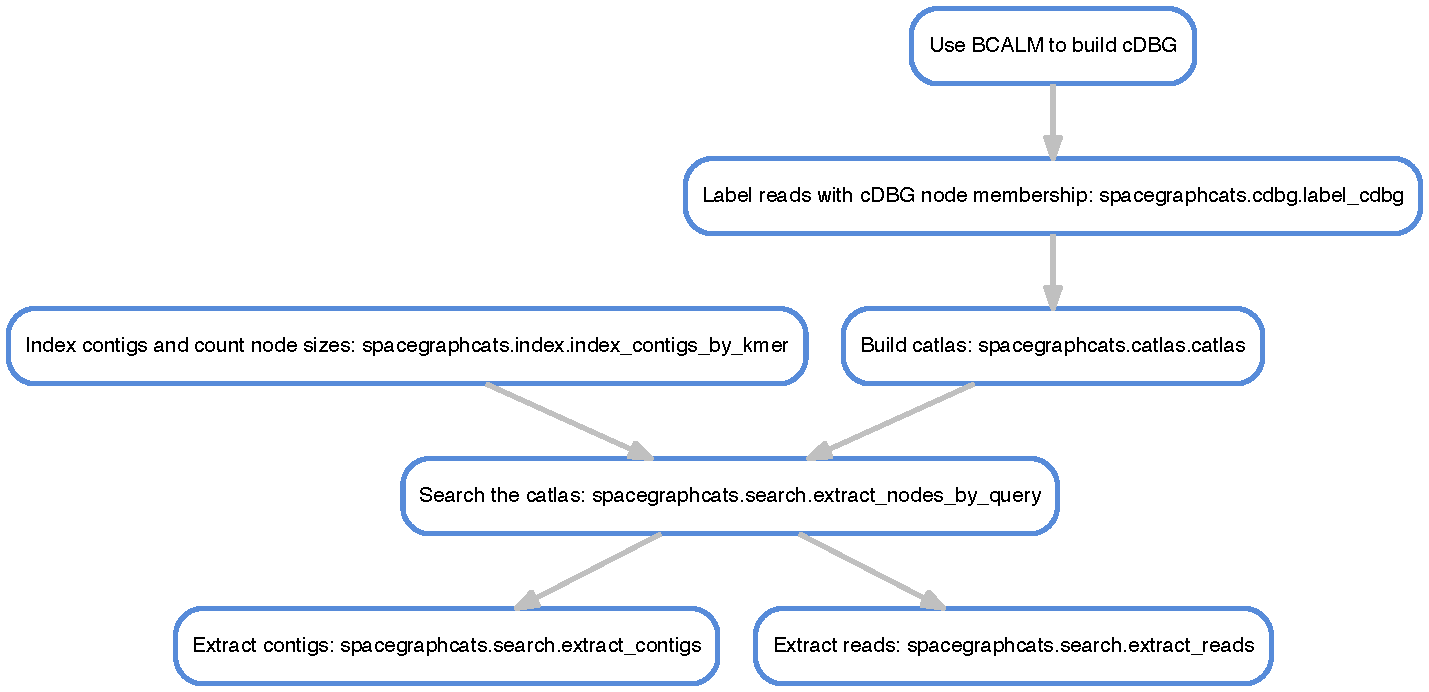
\includegraphics[width=\linewidth]{figures/sgc_dag}
	\caption{The steps followed by \textsf{spacegraphcats} when run
on sequencing data.
}
 \label{fig:sgc_dag}
\end{figure*}

\subsection{Query genome accession numbers for {\em Proteiniclasticum} search}
\label{subsec:query_accessions}

See Table~\ref{tab:query_accessions}.

\begin{table}[b]
  \begin{tabular}{l l c c }
    \toprule
    Name & NCBI accession \\
    \midrule
    \hline
    P. ruminis CGMCC & GCA\_900099635.1 \\
    P. ruminis DSM & GCA\_000701905.1 \\
    P. ruminis ML2 & GCA\_900115135.1 \\
    \hline
    \bottomrule
  \end{tabular}
  \caption{Accession numbers for genomes used in {\em Proteiniclasticum} neighborhood query.}
  \label{tab:query_accessions}
\end{table}

\subsection{Amino Acid Identity results for {\em Proteiniclasticum}}
\label{subsec:aai}

See Table~\ref{tab:aai}.

\begin{table}
  \begin{tabular}{l l c c }
    \toprule
    Genome A & Genome B & Orthologous Genes & Mean AAI \\
    \midrule
    {\em P. ruminis ML2} & {\em P. ruminis shakya} & 2546 & 95.74 \\
    {\em P. ruminis DSM} & {\em P. ruminis shakya}  & 2391 & 93.47 \\
    \hline
    \bottomrule
  \end{tabular}
  \caption{CompareM results for {\em Proteiniclasticum} genomes. {\em P. ruminis shakya} is the result of assembling the reads extracted from \podarv with the neighborhood search.}
  \label{tab:aai}
\end{table}


\subsection{\hu analysis pipeline overview}


See Figure~\ref{fig:hu_dag}. We implemented three workflows to analyze the
plass-assembled \hu query neighborhoods.


\begin{figure*}
 \centering
 \includegraphics[width=\linewidth]{figures/hu_dag}
	\caption{Three workflows implemented to analyze the plass-assembled
\hu query neighborhoods. The first three steps, depicted in blue, were common
across all workflows. The green boxes depict the KEGG GhostKOALA annotation
workflow, the results of which can be see in Figure~\ref{fig:hu_content}.
The orange boxes depict steps in common between the clustering and variant
workflows used to generate Figure~\ref{fig:hu_content}. The red boxes depict
steps used to generate the MDS clustering plot and the multiple sequence
alignment (see Figure~\ref{fig:gyrAalign}). The gold boxes depict the
steps of the variant workflow used to generate the assembly graphs.
}
 \label{fig:hu_dag}
\end{figure*}

\subsection{Genome bin completeness improvements for \hu}
\label{subsec:checkm}

See Table~\ref{tab:binstats} and
Table~\ref{tab:nbhdstats}. Table~\ref{tab:binstats} shows completeness metrics
for the binned genomes from the \hu sample and used as
queries.
Table~\ref{tab:nbhdstats} shows completeness metrics for \plass assembled
query neighborhoods after stringent read trimming at low abundance k-mers
(k-mers present fewer than 5 times were removed) of the SB1 sample reads.


\begin{table*}
  \begin{tabular}{l c c c c c c}
    \toprule
    Species & Completeness (\%) & Redundancy (\%) & Strain heterogeneity (\%) & Unique KOs & Size (bases) & Number of proteins \\
    \midrule
    M. bacterium 39\_7              & 50.06        & 5.94          & 0                    & 208        & 708389       & 657 \\
P. acetatigenes isolate 50\_10  & 56.68        & 3.6           & 66.67                & 506        & 1716233      & 1510 \\
WS6 bacterium 34\_10            & 61.85        & 29.47         & 61.29                & 219        & 1127556      & 1065 \\
Methanobacterium sp. 42\_16     & 97.6         & 0             & 0                    & 769        & 2173293      & 2149 \\
C. bacterium 38\_11             & 94.41        & 0.25          & 0                    & 825        & 1882878      & 1744 \\
Methanocalculus sp. 52\_23      & 82.71        & 4.58          & 66.67                & 689        & 1973787      & 2074 \\
A. bacterium 49\_20             & 69.55        & 8.28          & 0                    & 380        & 1023183      & 891 \\
M. infera isolate 46\_47        & 63.79        & 0.86          & 100                  & 502        & 1225111      & 1170 \\
WS6 bacterium 36\_33            & 31.52        & 6.48          & 85.71                & 127        & 439774       & 423 \\
P. bacterium 34\_609            & 34.03        & 1.1           & 12.5                 & 173        & 567617       & 557 \\
Desulfotomaculum sp. 46\_80     & 83.49        & 2.53          & 42.86                & 834        & 2251381      & 2148 \\
M. marisnigri isolate 62\_101   & 72.12        & 0.98          & 0                    & 583        & 1592820      & 1742 \\
S. bacterium 57\_84             & 90.83        & 1.85          & 50                   & 608        & 1255134      & 1277 \\
B. bacterium 38\_7              & 80.02        & 2.69          & 0                    & 601        & 2137321      & 1697 \\
S. bacterium 53\_16             & 91.53        & 4.24          & 0                    & 746        & 1772227      & 1741 \\
A. bacterium 34\_128            & 64.41        & 5.08          & 0                    & 423        & 894916       & 785 \\
M. bacterium 46\_47             & 72.89        & 0.1           & 0                    & 563        & 1629409      & 1413 \\
Desulfotomaculum sp. 46\_296    & 91.54        & 9.02          & 65.38                & 851        & 2328136      & 2265 \\
TA06 bacterium 32\_111          & 94.51        & 0             & 0                    & 619        & 1861827      & 1736 \\
P. bacterium 33\_209            & 47.86        & 5.17          & 0                    & 140        & 510490       & 526 \\
A. bacterium 66\_15             & 94.17        & 2.78          & 20                   & 811        & 2228088      & 2185 \\
A. thermophila isolate 46\_16   & 67.17        & 16.36         & 0                    & 474        & 1524726      & 1350 \\
M. harundinacea isolate 57\_489 & 100          & 0             & 0                    & 814        & 2382964      & 2377 \\              

\\
   \bottomrule
  \end{tabular}
  \caption{
   Completeness metrics for the \hu genome bins from \cite{Hu2016}, used as queries into the SB1 metagenome. Completeness, redundancy, and
   strain heterogeneity as estimated
   by checkM, unique KEGG orthologs predicted by GhostKOALA, bin size in
   bases, and number of prokka-predicted protein sequences in the \hu bins.
   Table is ordered by completeness. Note we refer to the checkM term
   ``contamination'' as ``redundancy'' as this better describes the calculated
   metric.}
  \label{tab:binstats}
 \end{table*}

\begin{table*}
  \begin{tabular}{l c c c c c c}
    \toprule
    Species & Completeness (\%) & Redundancy (\%) & Strain heterogeneity (\%) & Unique KOs & Size (bases) & Number of proteins \\
    \midrule
    WS6 bacterium 36\_33            & 45.7  & 1675.8 & 87.9 & 140 & 1206915  & 12990 \\
P. bacterium 34\_609            & 39.7 & 637.3   & 74.8 & 239 & 3604616  & 12372 \\
P. bacterium 33\_209            & 46.0 & 516.1  & 92.7 & 160 & 1830403  & 9836  \\
M. bacterium 39\_7              & 30.8 & 1.9    & 20    & 121 & 1356859  & 1208  \\
P. acetatigenes isolate 50\_10  & 42.7 & 66.3   & 86.7 & 557 & 6829683  & 6135  \\
WS6 bacterium 34\_10            & 58.6 & 352.8  & 86.0 & 219 & 2840498  & 6549  \\
M. infera isolate 46\_47        & 67.0 & 309.8   & 92.6  & 592 & 4021633  & 11798 \\
A. bacterium 34\_128            & 65.5 & 332     & 58.9 & 446 & 2703261  & 9030  \\
A. thermophila isolate 46\_16   & 60.5 & 250     & 88.5 & 457 & 5080416  & 13780 \\
A. bacterium 49\_20             & 71.3 & 187.2  & 76.7 & 392 & 4166615  & 6040  \\
M. marisnigri isolate 62\_101   & 82.2 & 1067.9 & 89.9 & 687 & 11380474 & 49119 \\
M. bacterium 46\_47             & 81.0 & 251.3  & 97.5  & 629 & 5308863  & 15964 \\
B. bacterium 38\_7              & 44.0 & 5.3    & 20    & 508 & 4229976  & 3901  \\
Methanocalculus sp. 52\_23      & 89.3 & 443.4  & 87.0 & 741 & 8018167  & 20999 \\
Desulfotomaculum sp. 46\_80     & 94.8 & 2327.3 & 94.7 & 858 & 7969109  & 48841 \\
S. bacterium 57\_84             & 90.8 & 598.2  & 83.9  & 686 & 5968936  & 24774 \\
S. bacterium 53\_16             & 94.0 & 95.6  & 83.9 & 786 & 7145072  & 12138 \\
Desulfotomaculum sp. 46\_296    & 94.8 & 2535.0 & 80.4 & 888 & 17836454 & 48174 \\
A. bacterium 66\_15             & 83.6 & 10.6   & 83.7 & 792 & 10865439 & 8152  \\
C. bacterium 38\_11             & 86.7 & 18.2   & 78.4 & 800 & 4932373  & 4582  \\
TA06 bacterium 32\_111          & 95.6  & 45.7   & 88.2  & 626 & 3811703  & 5724  \\
Methanobacterium sp. 42\_16     & 92.2 & 31.3   & 90.9 & 782 & 7007709  & 6335  \\
M. harundinacea isolate 57\_489 & 98.8 & 355.6  & 89.6 & 841 & 35722445 & 35093

\\
    \bottomrule
  \end{tabular}
  \caption{
   Completeness metrics for the query neighborhoods extracted from the \hu metagenome by {\sf spacegraphcats}. Completeness, redundancy,
   and strain heterogeneity as estimated
   by checkM, unique KEGG orthologs predicted by GhostKOALA, neighborhood
   size in  bases, and number of plass-assembled  protein sequences in the
   query neighborhoods. Table is ordered by completeness of query bins (see
   Table~\ref{tab:binstats}). All estimates were performed on the k-mer trimmed
   (k >= 5) \plass-assembled proteins except size of neighborhood in bases,
   for which we used the neighborhood unitig sequences output by {\sf spacegraphcats}.}
  \label{tab:nbhdstats}
 \end{table*}

\begin{table*}
% \parbox[t][][t]{.45\linewidth}{
 \begin{tabular}{@{}l l c c@{}}
    \toprule
    Species & gyrA (bin) & gyrA (\plass) \\
    \midrule
    % generated from notebook 'tables/plass-genes/distinct_positions.ipynb'
    Methanobacterium sp. 42\_16 & 0 & 0 \\
    P. bacterium 34\_609 & 0 & 0 \\
    Desulfotomaculum sp. 46\_80 & 0 & 0 \\
    S. bacterium 57\_84 & 0 & 0 \\
    B. bacterium & 0 & 1 \\
    P. acetatigenes isolate 50\_10 & 0 & 2 \\
    WS6 bacterium 34\_10 & 0 & 2 \\
    M. marisnigri isolate 62\_101 & 0 & 2 \\
    C. bacterium 38\_11 & 1 & 1 \\
    M. infera isolate 46\_47 & 1 & 1 \\
    S. bacterium 53\_16 & 1 & 1 \\
    M. bacterium 46\_47 & 1 & 1 \\
    TA06 bacterium 32\_111 & 1 & 1 \\
    P. bacterium 33\_209 & 1 & 1 \\
    A. bacterium 66\_15 & 1 & 1 \\
    Methanocalculus sp. 52\_23 & 1 & 2 \\
    WS6 bacterium 36\_33 & 1 & 2 \\
    A. bacterium 34\_128 & 1 & 2 \\
    A. thermophila isolate 46\_16 & 1 & 2 \\
    M. harundinacea isolate 57\_489 & 1 & 2 \\
    M. bacterium 39\_7 & 2 & 0 \\
    Desulfotomaculum sp. 46\_296 & 2 & 2 \\
    A. bacterium 49\_20 & 2 & 3 \\
    \bottomrule
  \end{tabular}
  \caption{
   Bin and neighborhood gyrA protein content. gyrA count for each bin is the number
    of gyrA amino acid sequences that are part of the original bin. gyrA count by \plass is
    the minimum number of gyrA amino acid sequences supported by at least one
    position with at least 10 copies of each variant, e.g. ``3'' indicates that
    there is at least one position in the multiple sequence alignment of gyrA
    sequences for that neighborhood that has 3 distinct variants in 10 distinct
    sequences.}
%    }
  \label{tab:gyrAcounts}
\end{table*}

\subsection{K-mer inclusion of reads by MEGAHIT assemblies}
\label{subsec:inclusion}

See Table~\ref{tab:kmer_inclusion}. We estimated the number of k-mers in each
query neighborhood that were contained in the MEGAHIT assembly of that query
neighborhood. We used sourmash {\tt compute} to calculate signatures with k-size of
31 and a scaled value of 2000. We then used sourmash {\tt compare} to estimate
containment in MEGAHIT assemblies. The query neighborhood with the smallest
containment, \emph{M. harundinacea} isolate \emph{57\_489}, had the largest query
neighborhood, while the query neighborhood with the largest containment,
\emph{M. bacterium 39\_7}, had the smallest query neighborhood.

\begin{table}
  \begin{tabular}{l c c}
    \toprule
    Species & MEGAHIT assembly containment & PLASS mapping \\
    \midrule
    % generated from notebook 'figures/megahit-assembly-inclusion.ipynb'
    M. harundinacea isolate 57\_489 & 4.2\% & 97.8\% \\
Desulfotomaculum sp. 46\_296 & 12.7\% & 97.7\% \\
M. marisnigri isolate 62\_101 & 13.6\% & 97.2\% \\
S. bacterium 57\_84 & 19.4\% & 97.9\% \\
P. bacterium 34\_609 & 19.7\% & 97.9\% \\
A. bacterium 66\_15 & 20.5\% & 96.9\% \\
Desulfotomaculum sp. 46\_80 & 24.1\% & 97.6\% \\
P. bacterium 33\_209 & 26.3\% & 97.6\% \\
S. bacterium 53\_16 & 30.9\% & 98.1\% \\
A. bacterium 49\_20 & 31.9\% & 96.9\% \\
Methanocalculus sp. 52\_23 & 33.4\% & 97.6\% \\
M. bacterium 46\_47 & 36.6\% & 98.4\% \\
P. acetatigenes isolate 50\_10 & 36.6\% & 97.1\% \\
A. bacterium 34\_128 & 36.8\% & 93.4\% \\
M. infera isolate 46\_47 & 38.0\% & 98.3\% \\
Methanobacterium sp. 42\_16 & 38.0\% & 95.2\% \\
A. thermophila isolate 46\_16 & 38.6\% & 95.9\% \\
TA06 bacterium 32\_111 & 44.1\% & 98.8\% \\
C. bacterium 38\_11 & 44.4\% & 96.0\% \\
WS6 bacterium 34\_10 & 53.2\% & 96.1\% \\
WS6 bacterium 36\_33 & 53.8\% & 98.2\% \\
B. bacterium & 54.2\% & 94.9\% \\
M. bacterium 39\_7 & 55.7\% & 95.6\% \\

%    M. bacterium 39\_7 & 0 & 0 \\
P. acetatigenes isolate 50\_10 & 0 & 0 \\
WS6 bacterium 34\_10 & 0 & 0 \\
Methanobacterium sp. 42\_16 & 0 & 0 \\
Methanocalculus sp. 52\_23 & 0 & 0 \\
WS6 bacterium 36\_33 & 0 & 0 \\
M. marisnigri isolate 62\_101 & 0 & 0 \\
B. bacterium & 0 & 0 \\
P. bacterium 33\_209 & 0 & 0 \\
M. harundinacea isolate 57\_489 & 0 & 0 \\
M. infera isolate 46\_47 & 0 & 1 \\
C. bacterium 38\_11 & 1 & 1 \\
A. bacterium 49\_20 & 1 & 1 \\
P. bacterium 34\_609 & 1 & 1 \\
S. bacterium 57\_84 & 1 & 1 \\
S. bacterium 53\_16 & 1 & 1 \\
A. bacterium 34\_128 & 1 & 1 \\
M. bacterium 46\_47 & 1 & 1 \\
TA06 bacterium 32\_111 & 1 & 1 \\
A. bacterium 66\_15 & 1 & 1 \\
A. thermophila isolate 46\_16 & 1 & 1 \\
Desulfotomaculum sp. 46\_80 & 1 & 2 \\
Desulfotomaculum sp. 46\_296 & 1 & 2 \\

    \bottomrule
  \end{tabular}
  \caption{Containment of neighborhood k-mer content in MEGAHIT nucleotide assemblies.}
  \label{tab:kmer_inclusion}
\end{table}

\subsection{gyrA alignment}
\label{subsec:gyrAalign}

See Figure~\ref{fig:gyrAalign}. The MDS plot in the left panel of figure 4 shows
distinct gyrA sequences identified in the Plass assemblies using HMMER. To visualize
the sequences within these clusters and in other query neighborhoods, we
constructed a multiple sequence alignment. However, because many
sequences assembled by Plass were fragmented (see Results: Some query neighborhoods
contain substantial strain variation), we first clustered the sequences at 95\%
similarity using CD-HIT. We then aligned the centroid sequences using MAFFT with
default settings. To produce the multiple sequence alignment visualization, we
calculated an unrooted neighbor joining tree using the MAFFT alignment. Then we used
the function {\tt msaplot} in the R package ggtree to plot the alignment.

\begin{figure*}
 \centering
 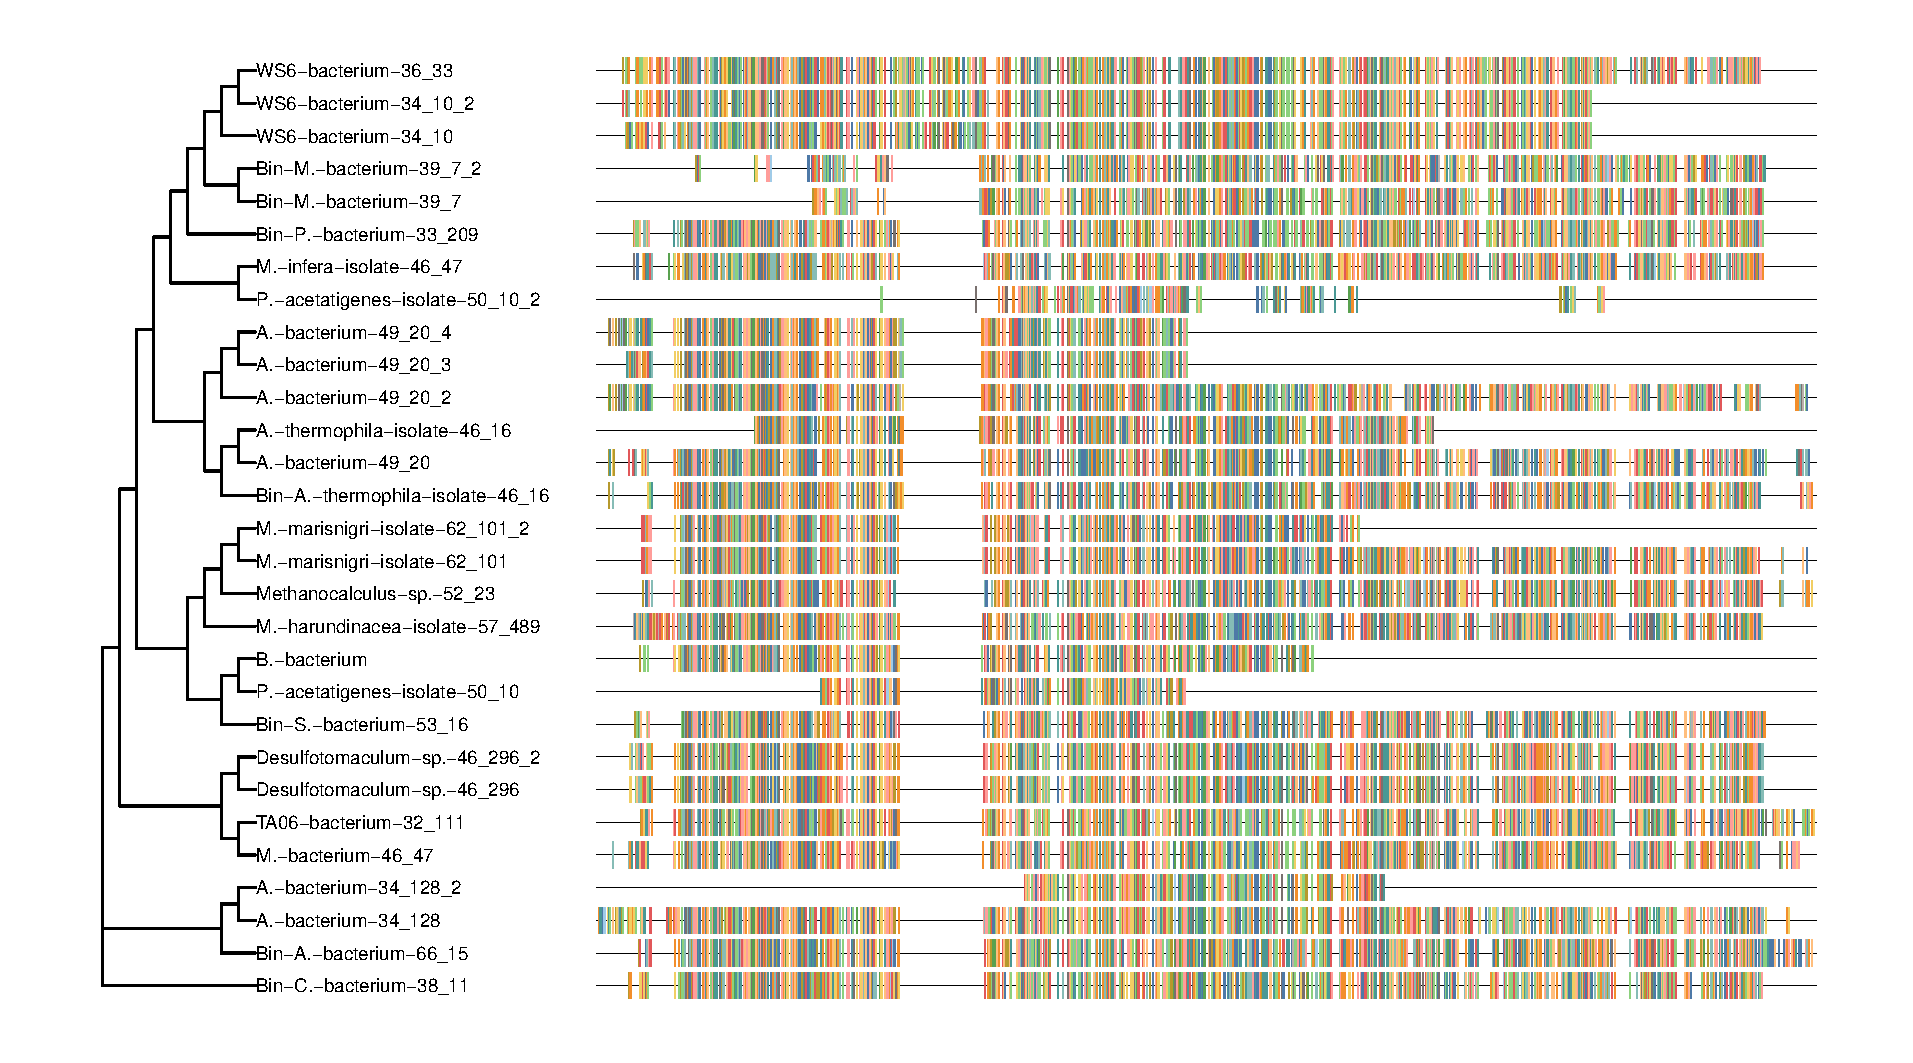
\includegraphics[width=\linewidth]{figures/gyrA-cdhit95-msa}
	\caption{A multiple sequence alignment and neighbor joining tree of representative gyrA amino acid fragments assembled by \plass from the genome neighborhoods in \hu. Protein sequences that originated from the genome bin are prepended with "Bin." All other sequences were assembled by Plass.
 }
 \label{fig:gyrAalign}
\end{figure*}

\subsection{gyrA by neighborhood}
\label{subsec:gyrAnbhd}

See Table~\ref{tab:gyrAcounts}. As can be seen in the left panel of Figure 4 in the
main text, we observe many unique amino acid sequences per single copy ortholog
per query neighborhood.
Although we observe many possible traversal paths in compact De Bruijn graphs built
from reads that give rise to these sequences, we have no way to ascertain whether we
observed combinatorial complexity by assembling variants that would never be linked
in nature. Therefore, we sought to conservatively estimate the number of positions
per amino acid sequence that contained variants using MAFFT alignments. First, we
subsetted the alignment to sequences from one query neighborhood. Then we identified
all aligned non-gap characters for each position in the alignment (gaps were induced
in some neighborhoods by the presence of amino acid residues in other query neighborhood
amino acid sequences). For each of these positions, we counted the number of unique
amino acid sequences per position, and the number of times each occurred at that position.
We then elimated any variant that occurred fewer than 10 times. Lastly, we counted the
number of well-supported distinct characters. We did this for gyrA, as well as the
amino acid sequences for the other genes we tested (see other genes). Table~\ref{tab:gyrAcounts}
shows that we see increased number of gyrA sequences in many neighborhoods even with
this conservative approach.

\subsection{Other genes}

\label{subsec:othergenes}

See bin and neighborhood content results for {\em alaS} in Table~\ref{tab:alaS}, {\em gyrB} in
Table~\ref{tab:gyrB}, {\em recA} in Table~\ref{tab:recA}, {\em rpb2d6} in Table~\ref{tab:rpb2d6},
rplB in Table~\ref{tab:rplB}, and rpsC in Table~\ref{tab:rpsC}. We selected {\em gyrB} and
{\em recA} because they were used by \hu to assign taxonomy to binned genomes. We selected
other genes used as single copy orthologs by programs like CheckM, and with longer PFAM
domains.


\newpage

\begin{table}
  \begin{tabular}{l l c c }
    \toprule
    Name & PFAM accession \\
    \midrule
    recA & PF00154 \\
    rplB & PF00181 \\
    rpsC & PF00189 \\
    gyrB & PF00204 \\
    gyrA & PF00521 \\
    rpb2d6 & PF00562 \\
    alaS & PF01411 \\
    \hline
    \bottomrule
  \end{tabular}
  \caption{Protein names and PFAM accessions for targeted analyses.}
  \label{tab:pfam_accessions}
\end{table}

\newpage

\begin{table}
  \begin{tabular}{l l c c }
    \toprule
    Species & alaS (bin) & alaS (\plass) \\
    \midrule
    % generated from notebook 'tables/plass-genes/distinct_positions.ipynb'
    P. acetatigenes isolate 50\_10 & 0 & 0 \\
A. bacterium 49\_20 & 0 & 0 \\
P. bacterium 34\_609 & 0 & 0 \\
B. bacterium & 0 & 0 \\
S. bacterium 53\_16 & 0 & 0 \\
A. bacterium 34\_128 & 0 & 0 \\
M. infera isolate 46\_47 & 0 & 2 \\
M. marisnigri isolate 62\_101 & 0 & 2 \\
M. bacterium 39\_7 & 1 & 0 \\
Methanobacterium sp. 42\_16 & 1 & 1 \\
C. bacterium 38\_11 & 1 & 1 \\
S. bacterium 57\_84 & 1 & 1 \\
TA06 bacterium 32\_111 & 1 & 1 \\
P. bacterium 33\_209 & 1 & 1 \\
A. bacterium 66\_15 & 1 & 1 \\
M. harundinacea isolate 57\_489 & 1 & 1 \\
Methanocalculus sp. 52\_23 & 1 & 2 \\
WS6 bacterium 36\_33 & 1 & 2 \\
Desulfotomaculum sp. 46\_80 & 1 & 2 \\
M. bacterium 46\_47 & 1 & 2 \\
Desulfotomaculum sp. 46\_296 & 1 & 2 \\
A. thermophila isolate 46\_16 & 2 & 1 \\
WS6 bacterium 34\_10 & 2 & 2 \\

    \bottomrule
  \end{tabular}
  \caption{Bin and neighborhood alaS protein content.}
  \label{tab:alaS}
\end{table}

\begin{table}
  \begin{tabular}{l l c c }
    \toprule
    Species & gyrB (bin) & gyrB (\plass) \\
    \midrule
    % generated from notebook 'tables/plass-genes/distinct_positions.ipynb'
    M. bacterium 39\_7 & 0 & 0 \\
P. acetatigenes isolate 50\_10 & 0 & 0 \\
Methanobacterium sp. 42\_16 & 0 & 0 \\
WS6 bacterium 36\_33 & 0 & 0 \\
P. bacterium 34\_609 & 0 & 0 \\
Desulfotomaculum sp. 46\_80 & 0 & 0 \\
S. bacterium 57\_84 & 0 & 0 \\
S. bacterium 53\_16 & 0 & 0 \\
A. thermophila isolate 46\_16 & 0 & 2 \\
P. bacterium 33\_209 & 1 & 0 \\
C. bacterium 38\_11 & 1 & 1 \\
M. infera isolate 46\_47 & 1 & 1 \\
M. bacterium 46\_47 & 1 & 1 \\
TA06 bacterium 32\_111 & 1 & 1 \\
A. bacterium 66\_15 & 1 & 1 \\
M. harundinacea isolate 57\_489 & 1 & 1 \\
WS6 bacterium 34\_10 & 1 & 2 \\
Methanocalculus sp. 52\_23 & 1 & 2 \\
M. marisnigri isolate 62\_101 & 1 & 2 \\
A. bacterium 34\_128 & 1 & 2 \\
A. bacterium 49\_20 & 2 & 2 \\
B. bacterium & 2 & 2 \\
Desulfotomaculum sp. 46\_296 & 2 & 2 \\

    \bottomrule
  \end{tabular}
  \caption{Bin and neighborhood gyrB protein content.}
  \label{tab:gyrB}
\end{table}

\begin{table}
  \begin{tabular}{l l c c }
    \toprule
    Species & recA (bin) & recA (\plass) \\
    \midrule
    % generated from notebook 'tables/plass-genes/distinct_positions.ipynb'
    M. bacterium 39\_7 & 0 & 0 \\
WS6 bacterium 34\_10 & 0 & 0 \\
Methanocalculus sp. 52\_23 & 0 & 0 \\
A. bacterium 49\_20 & 0 & 0 \\
WS6 bacterium 36\_33 & 0 & 0 \\
P. bacterium 34\_609 & 0 & 0 \\
M. marisnigri isolate 62\_101 & 0 & 0 \\
S. bacterium 53\_16 & 0 & 0 \\
M. bacterium 46\_47 & 0 & 0 \\
A. thermophila isolate 46\_16 & 0 & 1 \\
B. bacterium & 1 & 0 \\
P. acetatigenes isolate 50\_10 & 1 & 1 \\
Methanobacterium sp. 42\_16 & 1 & 1 \\
C. bacterium 38\_11 & 1 & 1 \\
M. infera isolate 46\_47 & 1 & 1 \\
S. bacterium 57\_84 & 1 & 1 \\
A. bacterium 34\_128 & 1 & 1 \\
TA06 bacterium 32\_111 & 1 & 1 \\
P. bacterium 33\_209 & 1 & 1 \\
A. bacterium 66\_15 & 1 & 1 \\
M. harundinacea isolate 57\_489 & 1 & 1 \\
Desulfotomaculum sp. 46\_80 & 1 & 2 \\
Desulfotomaculum sp. 46\_296 & 1 & 2 \\

    \bottomrule
  \end{tabular}
  \caption{Bin and neighborhood recA protein content.}
  \label{tab:recA}
\end{table}

\begin{table}
  \begin{tabular}{l l c c }
    \toprule
    Species & rpb2d6 (bin) & rpb2d6 (\plass) \\
    \midrule
    % generated from notebook 'tables/plass-genes/distinct_positions.ipynb'
    P. acetatigenes isolate 50\_10 & 0 & 0 \\
P. bacterium 34\_609 & 0 & 0 \\
S. bacterium 57\_84 & 0 & 1 \\
M. bacterium 46\_47 & 0 & 1 \\
C. bacterium 38\_11 & 1 & 0 \\
A. bacterium 49\_20 & 1 & 0 \\
M. bacterium 39\_7 & 1 & 1 \\
Methanobacterium sp. 42\_16 & 1 & 1 \\
Methanocalculus sp. 52\_23 & 1 & 1 \\
M. infera isolate 46\_47 & 1 & 1 \\
B. bacterium & 1 & 1 \\
S. bacterium 53\_16 & 1 & 1 \\
A. bacterium 34\_128 & 1 & 1 \\
TA06 bacterium 32\_111 & 1 & 1 \\
A. bacterium 66\_15 & 1 & 1 \\
A. thermophila isolate 46\_16 & 1 & 1 \\
WS6 bacterium 36\_33 & 1 & 2 \\
Desulfotomaculum sp. 46\_80 & 1 & 2 \\
M. marisnigri isolate 62\_101 & 1 & 2 \\
Desulfotomaculum sp. 46\_296 & 1 & 2 \\
P. bacterium 33\_209 & 1 & 2 \\
M. harundinacea isolate 57\_489 & 1 & 2 \\
WS6 bacterium 34\_10 & 2 & 2 \\

    \bottomrule
  \end{tabular}
  \caption{Bin and neighborhood rpb2d6 protein content.}
  \label{tab:rpb2d6}
\end{table}

\begin{table}
  \begin{tabular}{l l c c }
    \toprule
    Species & rplB (bin) & rplB (\plass) \\
    \midrule
    % generated from notebook 'tables/plass-genes/distinct_positions.ipynb'
    M. bacterium 39\_7 & 0 & 0 \\
Methanobacterium sp. 42\_16 & 0 & 0 \\
Methanocalculus sp. 52\_23 & 0 & 0 \\
WS6 bacterium 36\_33 & 0 & 0 \\
M. marisnigri isolate 62\_101 & 0 & 0 \\
M. harundinacea isolate 57\_489 & 0 & 0 \\
P. acetatigenes isolate 50\_10 & 1 & 1 \\
C. bacterium 38\_11 & 1 & 1 \\
A. bacterium 49\_20 & 1 & 1 \\
M. infera isolate 46\_47 & 1 & 1 \\
P. bacterium 34\_609 & 1 & 1 \\
Desulfotomaculum sp. 46\_80 & 1 & 1 \\
S. bacterium 57\_84 & 1 & 1 \\
B. bacterium & 1 & 1 \\
S. bacterium 53\_16 & 1 & 1 \\
A. bacterium 34\_128 & 1 & 1 \\
M. bacterium 46\_47 & 1 & 1 \\
Desulfotomaculum sp. 46\_296 & 1 & 1 \\
TA06 bacterium 32\_111 & 1 & 1 \\
P. bacterium 33\_209 & 1 & 1 \\
A. bacterium 66\_15 & 1 & 1 \\
A. thermophila isolate 46\_16 & 1 & 1 \\
WS6 bacterium 34\_10 & 1 & 2 \\

    \bottomrule
  \end{tabular}
  \caption{Bin and neighborhood rplB protein content.}
  \label{tab:rplB}
\end{table}

\begin{table}
  \begin{tabular}{l l c c }
    \toprule
    Species & rpsC (bin) & rpsC (\plass) \\
    \midrule
    % generated from notebook 'tables/plass-genes/distinct_positions.ipynb'
    M. bacterium 39\_7 & 0 & 0 \\
P. acetatigenes isolate 50\_10 & 0 & 0 \\
WS6 bacterium 34\_10 & 0 & 0 \\
Methanobacterium sp. 42\_16 & 0 & 0 \\
Methanocalculus sp. 52\_23 & 0 & 0 \\
WS6 bacterium 36\_33 & 0 & 0 \\
M. marisnigri isolate 62\_101 & 0 & 0 \\
B. bacterium & 0 & 0 \\
P. bacterium 33\_209 & 0 & 0 \\
M. harundinacea isolate 57\_489 & 0 & 0 \\
M. infera isolate 46\_47 & 0 & 1 \\
C. bacterium 38\_11 & 1 & 1 \\
A. bacterium 49\_20 & 1 & 1 \\
P. bacterium 34\_609 & 1 & 1 \\
S. bacterium 57\_84 & 1 & 1 \\
S. bacterium 53\_16 & 1 & 1 \\
A. bacterium 34\_128 & 1 & 1 \\
M. bacterium 46\_47 & 1 & 1 \\
TA06 bacterium 32\_111 & 1 & 1 \\
A. bacterium 66\_15 & 1 & 1 \\
A. thermophila isolate 46\_16 & 1 & 1 \\
Desulfotomaculum sp. 46\_80 & 1 & 2 \\
Desulfotomaculum sp. 46\_296 & 1 & 2 \\

    \bottomrule
  \end{tabular}
  \caption{Bin and neighborhood rpsC protein content.}
  \label{tab:rpsC}
\end{table}

\newpage

\begin{table}
  \begin{tabular}{l c c}
    \toprule
    Species & MEGAHIT assembly containment & PLASS mapping \\
    \midrule
    % generated from notebook 'figures/megahit-assembly-inclusion.ipynb'
    M. harundinacea isolate 57\_489 & 4.2\% & 97.8\% \\
Desulfotomaculum sp. 46\_296 & 12.7\% & 97.7\% \\
M. marisnigri isolate 62\_101 & 13.6\% & 97.2\% \\
S. bacterium 57\_84 & 19.4\% & 97.9\% \\
P. bacterium 34\_609 & 19.7\% & 97.9\% \\
A. bacterium 66\_15 & 20.5\% & 96.9\% \\
Desulfotomaculum sp. 46\_80 & 24.1\% & 97.6\% \\
P. bacterium 33\_209 & 26.3\% & 97.6\% \\
S. bacterium 53\_16 & 30.9\% & 98.1\% \\
A. bacterium 49\_20 & 31.9\% & 96.9\% \\
Methanocalculus sp. 52\_23 & 33.4\% & 97.6\% \\
M. bacterium 46\_47 & 36.6\% & 98.4\% \\
P. acetatigenes isolate 50\_10 & 36.6\% & 97.1\% \\
A. bacterium 34\_128 & 36.8\% & 93.4\% \\
M. infera isolate 46\_47 & 38.0\% & 98.3\% \\
Methanobacterium sp. 42\_16 & 38.0\% & 95.2\% \\
A. thermophila isolate 46\_16 & 38.6\% & 95.9\% \\
TA06 bacterium 32\_111 & 44.1\% & 98.8\% \\
C. bacterium 38\_11 & 44.4\% & 96.0\% \\
WS6 bacterium 34\_10 & 53.2\% & 96.1\% \\
WS6 bacterium 36\_33 & 53.8\% & 98.2\% \\
B. bacterium & 54.2\% & 94.9\% \\
M. bacterium 39\_7 & 55.7\% & 95.6\% \\

%    M. bacterium 39\_7 & 0 & 0 \\
P. acetatigenes isolate 50\_10 & 0 & 0 \\
WS6 bacterium 34\_10 & 0 & 0 \\
Methanobacterium sp. 42\_16 & 0 & 0 \\
Methanocalculus sp. 52\_23 & 0 & 0 \\
WS6 bacterium 36\_33 & 0 & 0 \\
M. marisnigri isolate 62\_101 & 0 & 0 \\
B. bacterium & 0 & 0 \\
P. bacterium 33\_209 & 0 & 0 \\
M. harundinacea isolate 57\_489 & 0 & 0 \\
M. infera isolate 46\_47 & 0 & 1 \\
C. bacterium 38\_11 & 1 & 1 \\
A. bacterium 49\_20 & 1 & 1 \\
P. bacterium 34\_609 & 1 & 1 \\
S. bacterium 57\_84 & 1 & 1 \\
S. bacterium 53\_16 & 1 & 1 \\
A. bacterium 34\_128 & 1 & 1 \\
M. bacterium 46\_47 & 1 & 1 \\
TA06 bacterium 32\_111 & 1 & 1 \\
A. bacterium 66\_15 & 1 & 1 \\
A. thermophila isolate 46\_16 & 1 & 1 \\
Desulfotomaculum sp. 46\_80 & 1 & 2 \\
Desulfotomaculum sp. 46\_296 & 1 & 2 \\

    \bottomrule
  \end{tabular}
  \caption{Containment of neighborhood k-mer content in MEGAHIT nucleotide assemblies.}
  \label{tab:kmer_inclusion}
\end{table}


\end{document}
